\chapter{Gráficos dos Experimentos}
\label{ape:graphics}

%Aqui são mostrados os gráficos de cada uma das repetições dos experimentos, para os dois algoritmos de balanceamento de carga.

%colocar todas as figuras do mesmo algoritmo na mesma pagina
%\section{Experimento 1 - Algoritmo de Uso de Estado}

%\subsection{Vazão}


\begin{figure}[h]
\centering
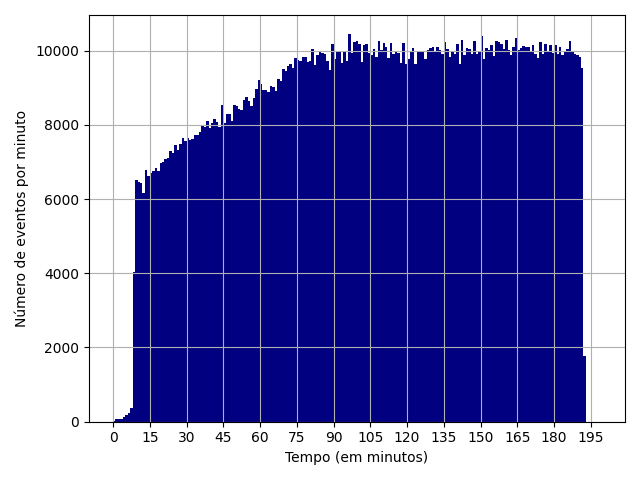
\includegraphics[width=\textwidth]{figuras/graphics/histogram_vazao_5-dez-su.png}
\caption{Vazão de eventos detectados pelo sistema na execução 1 do experimento utilizando o algoritmo de balanceamento por Uso de Estado.}
\label{fig:vazao_5-dez-su}
\end{figure}

%\subsection{Número de instâncias e de eventos de entrada}


\begin{figure}[h]
\centering
\vspace{5cm}
\begin{subfigure}{0.9\textwidth}
\centering
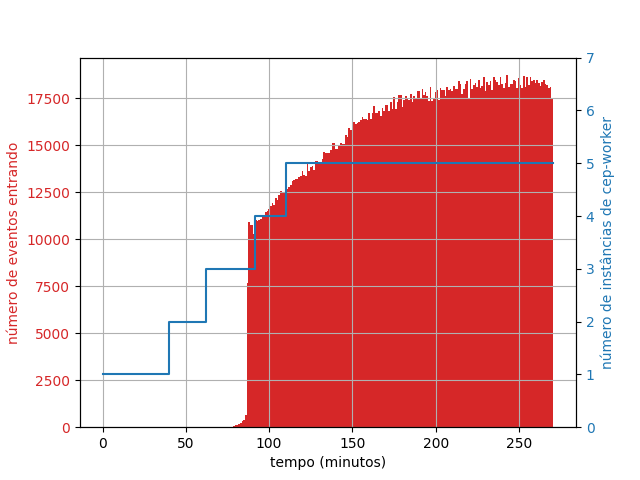
\includegraphics[width=0.8\textwidth]{figuras/graphics/carga_e_workers_total5-dez-su.png}
\caption{Número de eventos entrando no sistema (em vermelho) e número de instâncias de \texttt{CEP Worker} (em azul) em função do tempo na execução 1 do experimento utilizando o algoritmo de balanceamento de carga por Uso de Estado.}
\label{fig:workers_and_load_total}
\end{subfigure}%

\begin{subfigure}{\textwidth}
\centering
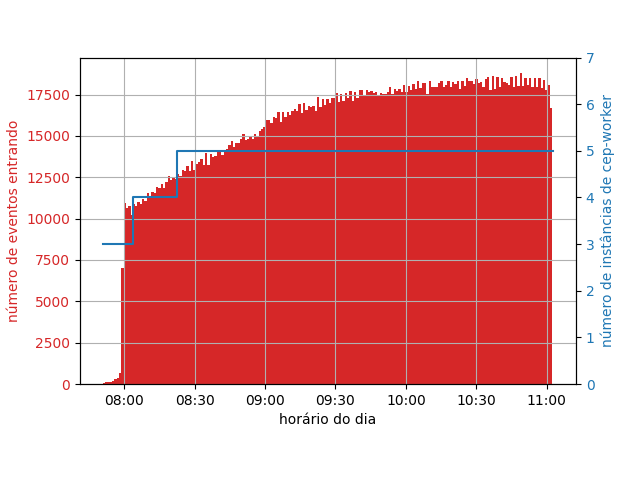
\includegraphics[width=\textwidth]{figuras/graphics/carga_e_workers_horario5-dez-su.png}
\caption{Número de eventos entrando no sistema (em vermelho) e número de instâncias de \texttt{CEP Worker} (em azul) em função do horário do dia na execução 1 do experimento utilizando o algoritmo de balanceamento de carga por Uso de Estado.}
\label{fig:workers_and_load_SPtrans}
\end{subfigure}%
\caption{Número de eventos entrando no sistema e número de instâncias de \texttt{CEP Worker} na execução 1 do experimento utilizando o algoritmo de balanceamento de carga por Uso de Estado.}
\end{figure}

%\subsection{Latência}


\begin{figure}
\centering
\begin{subfigure}{.5\textwidth}
\centering
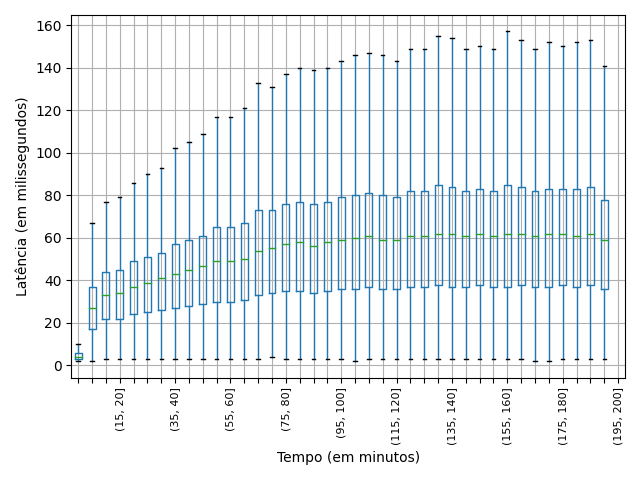
\includegraphics[width=\textwidth]{figuras/graphics/boxplot_5-dez-su_vf.png}
\caption{BoxPlot da latência da categoria de tipos de evento \textbf{vf} por intervalos de cinco minutos ao longo da execução 1 do experimento utilizando o algoritmo de balanceamento de carga por Uso de Estado.}
\label{fig:BoxPlot_vf_SU_1}
\end{subfigure}%
%\end{figure}

%\begin{figure}
\begin{subfigure}{.5\textwidth}
\centering
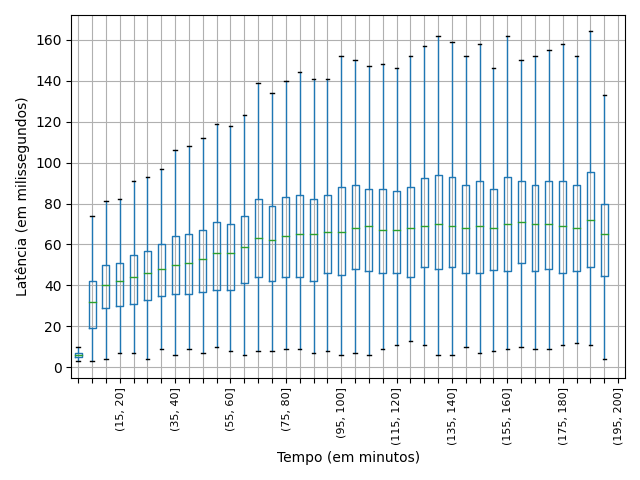
\includegraphics[width=\textwidth]{figuras/graphics/boxplot_5-dez-su_vi.png}
\caption{BoxPlot da latência da categoria de tipos de evento \textbf{vi} por intervalos de cinco minutos ao longo da execução 1 do experimento utilizando o algoritmo de balanceamento de carga por Uso de Estado.}
\label{fig:BoxPlot_vi_SU_1}
\end{subfigure}%
%\end{figure}
\centering
%\begin{figure}
\begin{subfigure}{.5\textwidth}
\centering
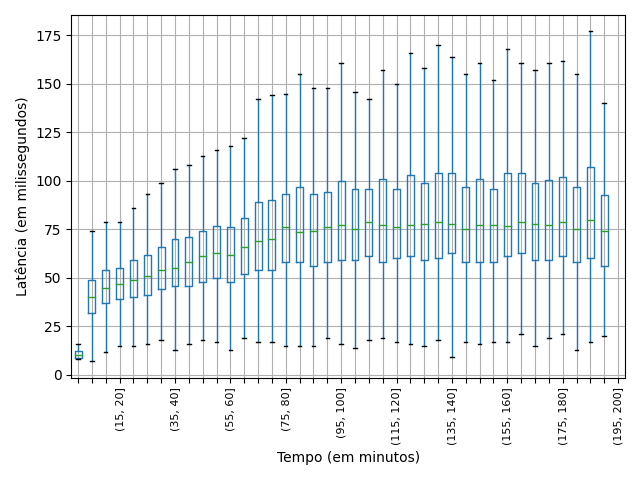
\includegraphics[width=\textwidth]{figuras/graphics/boxplot_5-dez-su_vel.png}
\caption{BoxPlot da latência da categoria de tipos de evento \textbf{vel} por intervalos de cinco minutos ao longo da execução 1 do experimento utilizando o algoritmo de balanceamento de carga por Uso de Estado.}
\label{fig:BoxPlot_vel_SU_1}
\end{subfigure}%
%\end{figure}

%\begin{figure}
\begin{subfigure}{.5\textwidth}
\centering
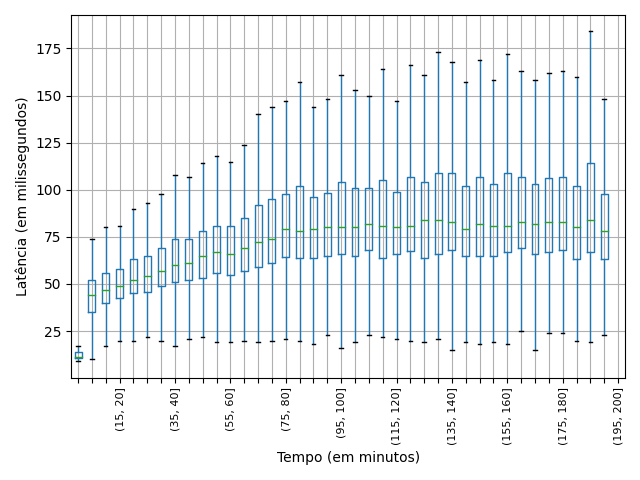
\includegraphics[width=\textwidth]{figuras/graphics/boxplot_5-dez-su_corr.png}
\caption{BoxPlot da latência da categoria de tipos de evento \textbf{corr} por intervalos de cinco minutos ao longo da execução 1 do experimento utilizando o algoritmo de balanceamento de carga por Uso de Estado.}
\label{fig:BoxPlot_corr_SU_1}
\end{subfigure}%
%\end{figure}
%\begin{figure}
\begin{subfigure}{.5\textwidth}
\centering
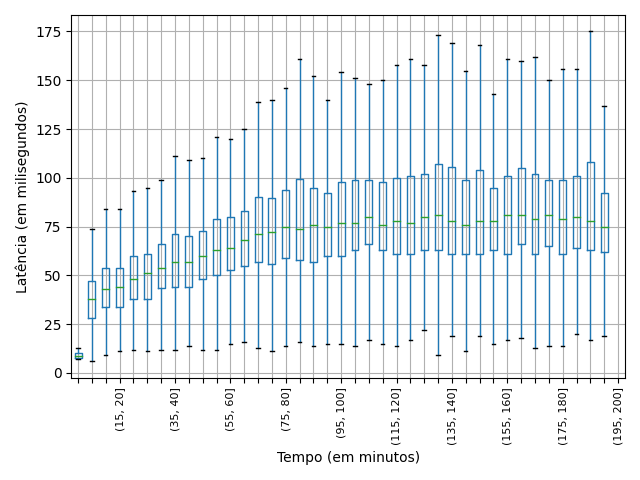
\includegraphics[width=\textwidth]{figuras/graphics/boxplot_5-dez-su_busb.png}
\caption{BoxPlot da latência da categoria de tipos de evento \textbf{BusB} por intervalos de cinco minutos ao longo da execução 1 do experimento utilizando o algoritmo de balanceamento de carga por Uso de Estado.}
\label{fig:BoxPlot_BusB_SU_1}
\end{subfigure}%
\caption{BoxPlot da latência por intervalos de cinco minutos ao longo da execução 1 do experimento utilizando o algoritmo de balanceamento de carga por Uso de Estado.}
\end{figure}






%----------------------------------------
%\newpage
%\section{Experimento 1 - Algoritmo de Similaridade de Entrada}


%\subsection{Vazão}


\begin{figure}[h]
\centering
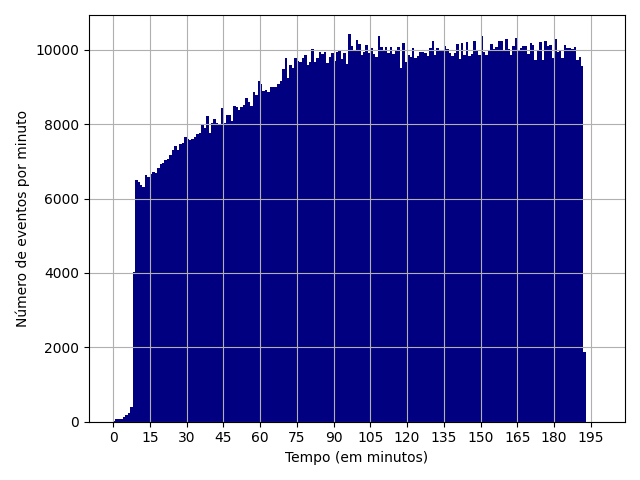
\includegraphics[width=\textwidth]{figuras/graphics/histogram_vazao_6-dez-is.png}
\caption{Vazão de eventos detectados pelo sistema na execução 1 do experimento utilizando o algoritmo de balanceamento por Similaridade de Entrada.}
\label{fig:vazao_6-dez-is}
\end{figure}

%\subsection{Número de instâncias e de eventos de entrada}


\begin{figure}[h]
\centering
\begin{subfigure}{0.9\textwidth}
\centering
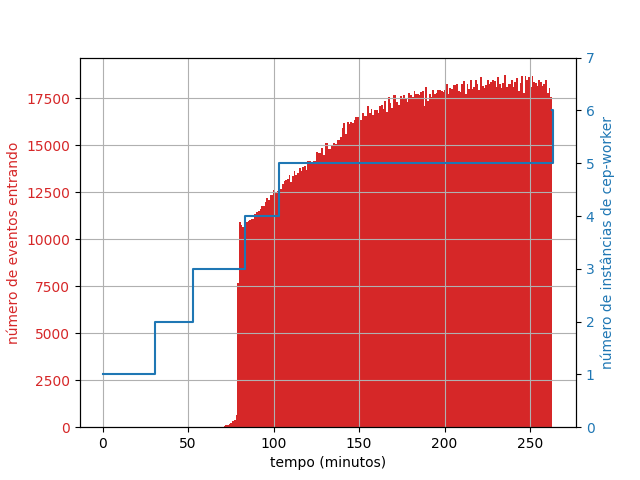
\includegraphics[width=\textwidth]{figuras/graphics/carga_e_workers_total6-dez-is.png}
\caption{Número de eventos entrando no sistema (em vermelho) e número de instâncias de \texttt{CEP Worker} (em azul) em função do tempo na execução 1 do experimento utilizando o algoritmo de balanceamento de carga por Similaridade de Entrada.}
\label{fig:workers_and_load_total-6-dez-is}
\end{subfigure}%

\begin{subfigure}{\textwidth}
\centering
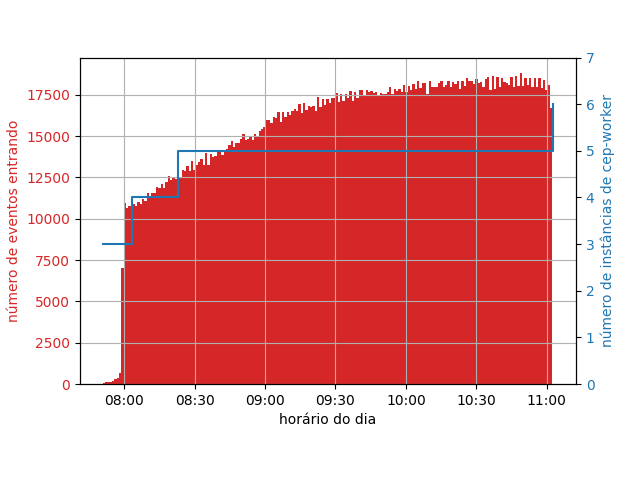
\includegraphics[width=\textwidth]{figuras/graphics/carga_e_workers_horario6-dez-is.png}
\caption{Número de eventos entrando no sistema (em vermelho) e número de instâncias de \texttt{CEP Worker} (em azul) em função do horário do dia na execução 1 do experimento utilizando o algoritmo de balanceamento de carga por Similaridade de Entrada.}
\label{fig:workers_and_load_SPtrans-6-dez-is}
\end{subfigure}%
\caption{Número de eventos entrando no sistema e número de instâncias de \texttt{CEP Worker} na execução 1 do experimento utilizando o algoritmo de balanceamento de carga por Similaridade de Entrada.}
\end{figure}



%\subsection{Latência}


\begin{figure}
\centering
\begin{subfigure}{.5\textwidth}
\centering
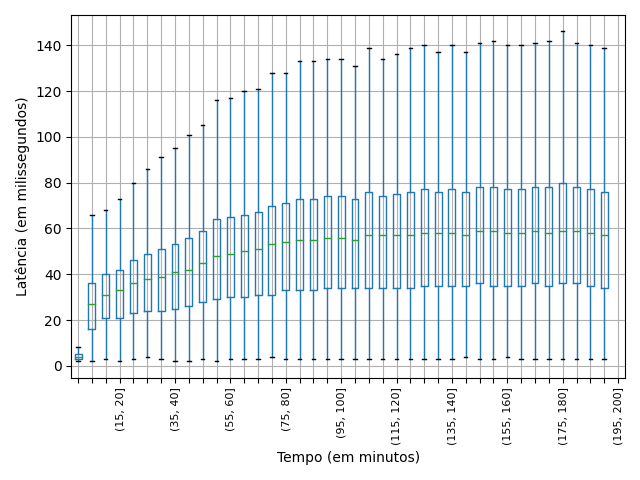
\includegraphics[width=\textwidth]{figuras/graphics/boxplot_6-dez-is_vf.png}
\caption{BoxPlot da latência da categoria de tipos de evento \textbf{vf} por intervalos de cinco minutos ao longo da execução 1 do experimento utilizando o algoritmo de balanceamento de carga por Similaridade de Entrada.}
\label{fig:BoxPlot_vf_IS_1}
\end{subfigure}%
%\end{figure}

%\begin{figure}
\begin{subfigure}{.5\textwidth}
\centering
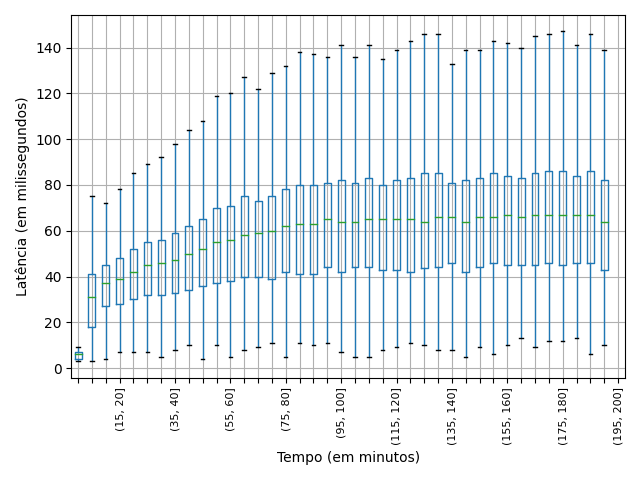
\includegraphics[width=\textwidth]{figuras/graphics/boxplot_6-dez-is_vi.png}
\caption{BoxPlot da latência da categoria de tipos de evento \textbf{vi} por intervalos de cinco minutos ao longo da execução 1 do experimento utilizando o algoritmo de balanceamento de carga por Similaridade de Entrada.}
\label{fig:BoxPlot_vi_IS_1}
\end{subfigure}%
%\end{figure}
\centering
%\begin{figure}
\begin{subfigure}{.5\textwidth}
\centering
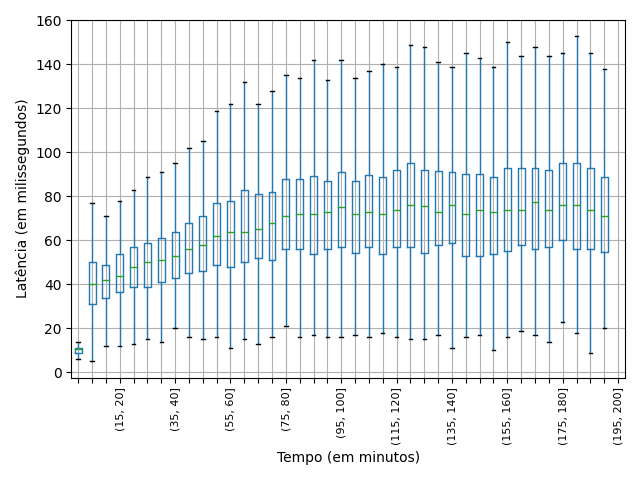
\includegraphics[width=\textwidth]{figuras/graphics/boxplot_6-dez-is_vel.png}
\caption{BoxPlot da latência da categoria de tipos de evento \textbf{vel} por intervalos de cinco minutos ao longo da execução 1 do experimento utilizando o algoritmo de balanceamento de carga por Similaridade de Entrada.}
\label{fig:BoxPlot_vel_IS_1}
\end{subfigure}%
%\end{figure}

%\begin{figure}
\begin{subfigure}{.5\textwidth}
\centering
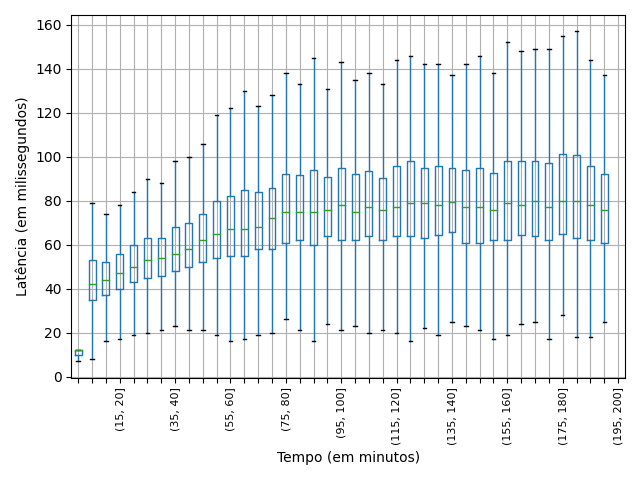
\includegraphics[width=\textwidth]{figuras/graphics/boxplot_6-dez-is_corr.png}
\caption{BoxPlot da latência da categoria de tipos de evento \textbf{corr} por intervalos de cinco minutos ao longo da execução 1 do experimento utilizando o algoritmo de balanceamento de carga por Similaridade de Entrada.}
\label{fig:BoxPlot_corr_IS_1}
\end{subfigure}%
%\end{figure}
%\begin{figure}
\begin{subfigure}{.5\textwidth}
\centering
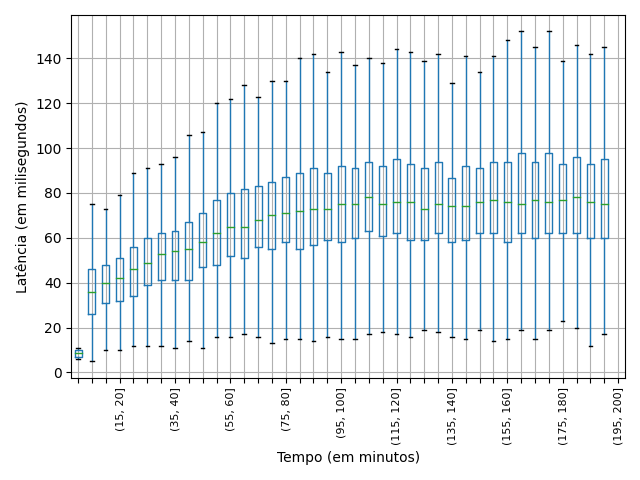
\includegraphics[width=\textwidth]{figuras/graphics/boxplot_6-dez-is_busb.png}
\caption{BoxPlot da latência da categoria de tipos de evento \textbf{BusB} por intervalos de cinco minutos ao longo da execução 1 do experimento utilizando o algoritmo de balanceamento de carga por Similaridade de Entrada.}
\label{fig:BoxPlot_BusB_IS_1}
\end{subfigure}%
\caption{BoxPlot da latência por intervalos de cinco minutos ao longo da execução 1 do experimento utilizando o algoritmo de balanceamento de carga por Similaridade de Entrada.}
\end{figure}




%\newpage

%------------------------------------------------

%\section{Experimento 2 - Algoritmo de Uso de Estado}

%\subsection{Vazão}


\begin{figure}[h]
\centering
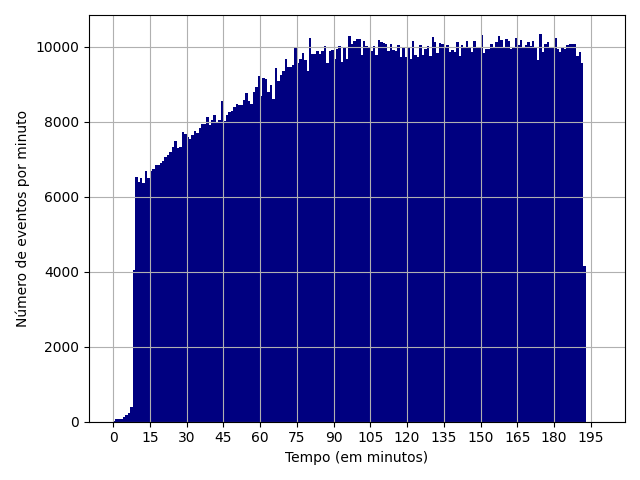
\includegraphics[width=\textwidth]{figuras/graphics/histogram_vazao_7-dez-su.png}
\caption{Vazão de eventos detectados pelo sistema na execução 2 do experimento utilizando o algoritmo de balanceamento por Uso de Estado.}
\label{fig:vazao_7-dez-su}
\end{figure}


%\subsection{Número de instâncias e de eventos de entrada}


\begin{figure}[h]
\centering
\begin{subfigure}{0.9\textwidth}
\centering
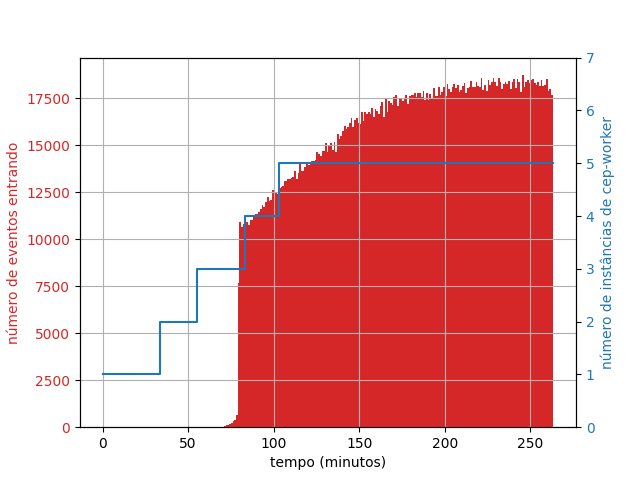
\includegraphics[width=\textwidth]{figuras/graphics/carga_e_workers_total7-dez-su.png}
\caption{Número de eventos entrando no sistema (em vermelho) e número de instâncias de \texttt{CEP Worker} (em azul) em função do tempo na execução 2 do experimento utilizando o algoritmo de balanceamento de carga por Uso de Estado.}
\label{fig:workers_and_load_total_7-dez-su}
\end{subfigure}%

\begin{subfigure}{\textwidth}
\centering
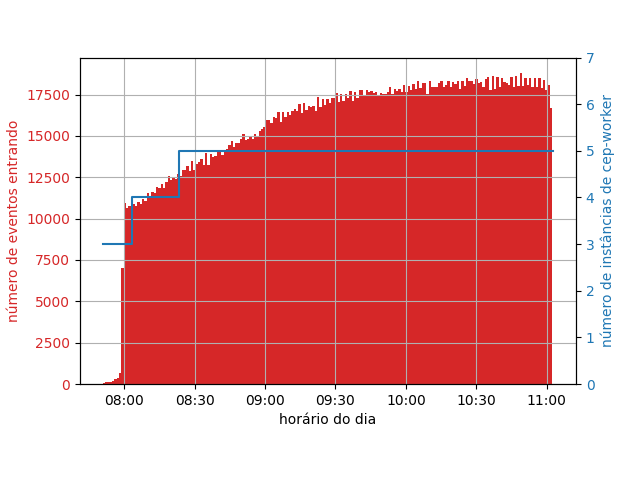
\includegraphics[width=\textwidth]{figuras/graphics/carga_e_workers_horario7-dez-su.png}
\caption{Número de eventos entrando no sistema (em vermelho) e número de instâncias de \texttt{CEP Worker} (em azul) em função do horário do dia na execução 2 do experimento utilizando o algoritmo de balanceamento de carga por Uso de Estado.}
\label{fig:workers_and_load_SPtrans_7-dez-su}
\end{subfigure}%
\caption{Número de eventos entrando no sistema e número de instâncias de \texttt{CEP Worker} na execução 2 do experimento utilizando o algoritmo de balanceamento de carga por Uso de Estado.}
\end{figure}


%\subsection{Latência}


\begin{figure}
\centering
\begin{subfigure}{.5\textwidth}
\centering
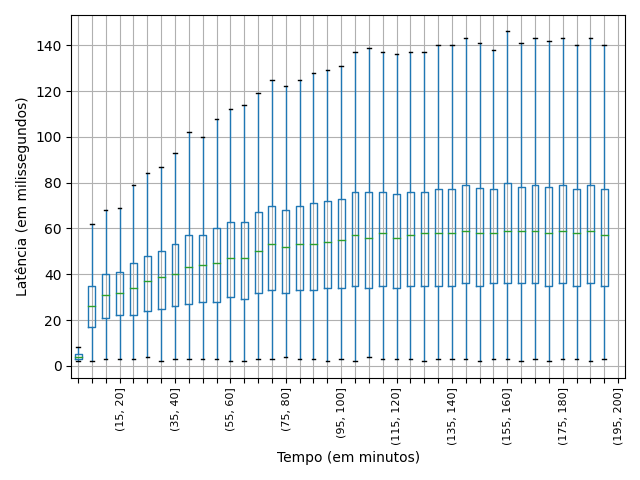
\includegraphics[width=\textwidth]{figuras/graphics/boxplot_7-dez-su_vf.png}
\caption{BoxPlot da latência da categoria de tipos de evento \textbf{vf} por intervalos de cinco minutos ao longo da execução 2 do experimento utilizando o algoritmo de balanceamento de carga por Uso de Estado.}
\label{fig:BoxPlot_vf_SU_7-dez-su}
\end{subfigure}%
%\end{figure}

%\begin{figure}
\begin{subfigure}{.5\textwidth}
\centering
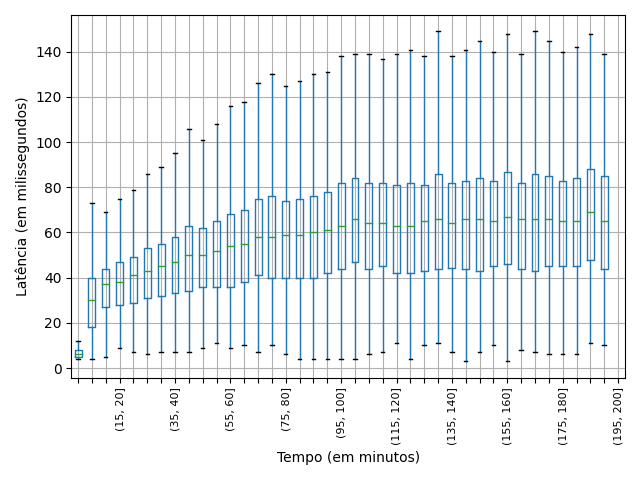
\includegraphics[width=\textwidth]{figuras/graphics/boxplot_7-dez-su_vi.png}
\caption{BoxPlot da latência da categoria de tipos de evento \textbf{vi} por intervalos de cinco minutos ao longo da execução 2 do experimento utilizando o algoritmo de balanceamento de carga por Uso de Estado.}
\label{fig:BoxPlot_vi_SU_7-dez-su}
\end{subfigure}%
%\end{figure}
\centering
%\begin{figure}
\begin{subfigure}{.5\textwidth}
\centering
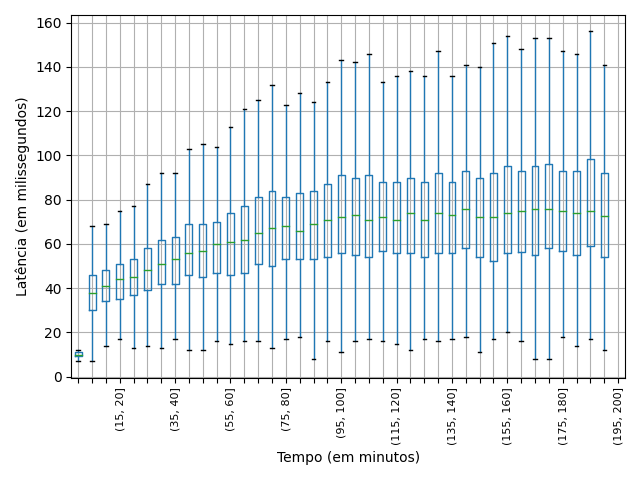
\includegraphics[width=\textwidth]{figuras/graphics/boxplot_7-dez-su_vel.png}
\caption{BoxPlot da latência da categoria de tipos de evento \textbf{vel} por intervalos de cinco minutos ao longo da execução 2 do experimento utilizando o algoritmo de balanceamento de carga por Uso de Estado.}
\label{fig:BoxPlot_vel_SU_7-dez-su}
\end{subfigure}%
%\end{figure}

%\begin{figure}
\begin{subfigure}{.5\textwidth}
\centering
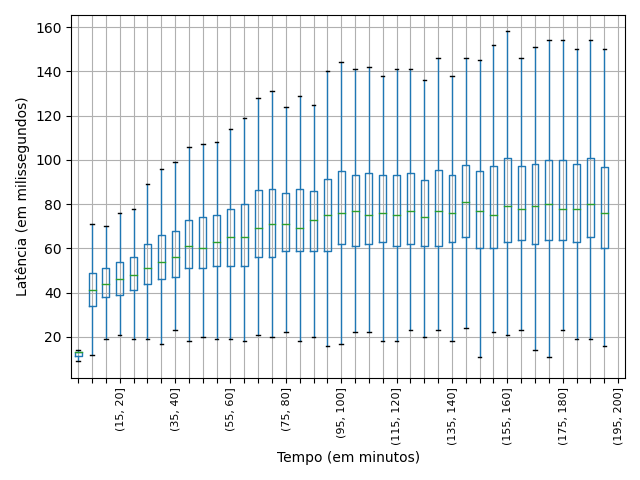
\includegraphics[width=\textwidth]{figuras/graphics/boxplot_7-dez-su_corr.png}
\caption{BoxPlot da latência da categoria de tipos de evento \textbf{corr} por intervalos de cinco minutos ao longo da execução 2 do experimento utilizando o algoritmo de balanceamento de carga por Uso de Estado.}
\label{fig:BoxPlot_corr_SU_7-dez-su}
\end{subfigure}%
%\end{figure}
%\begin{figure}
\begin{subfigure}{.5\textwidth}
\centering
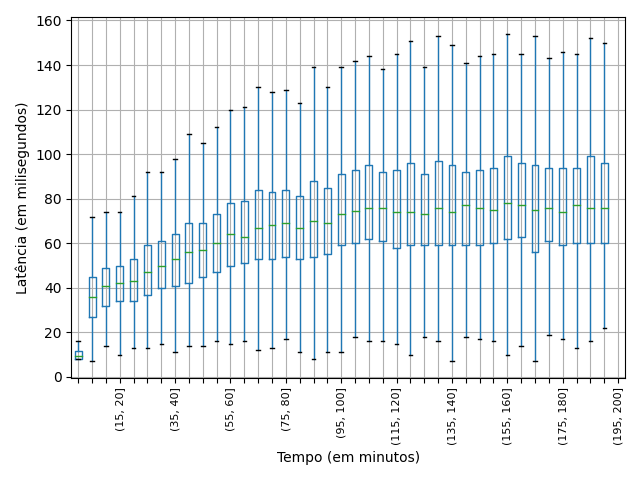
\includegraphics[width=\textwidth]{figuras/graphics/boxplot_7-dez-su_busb.png}
\caption{BoxPlot da latência da categoria de tipos de evento \textbf{BusB} por intervalos de cinco minutos ao longo da execução 2 do experimento utilizando o algoritmo de balanceamento de carga por Uso de Estado.}
\label{fig:BoxPlot_BusB_SU_7-dez-su}
\end{subfigure}%
\caption{BoxPlot da latência por intervalos de cinco minutos ao longo da execução 2 do experimento utilizando o algoritmo de balanceamento de carga por Uso de Estado.}
\end{figure}






%----------------------------------------
%\newpage
%\section{Experimento 2 - Algoritmo de Similaridade de Entrada}

%\subsection{Vazão}


\begin{figure}[h]
\centering
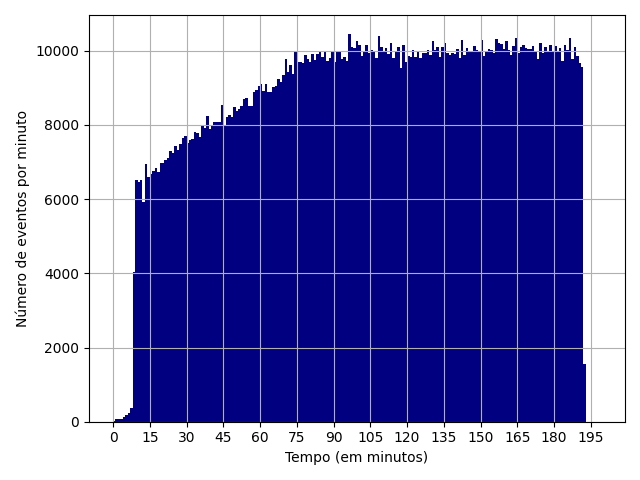
\includegraphics[width=\textwidth]{figuras/graphics/histogram_vazao_7-dez-is.png}
\caption{Vazão de eventos detectados pelo sistema na execução 2 do experimento utilizando o algoritmo de balanceamento por Similaridade de Entrada.}
\label{fig:vazao_7-dez-is}
\end{figure}

%\subsection{Número de instâncias e de eventos de entrada}


\begin{figure}[h]
\centering
\begin{subfigure}{0.9\textwidth}
\centering
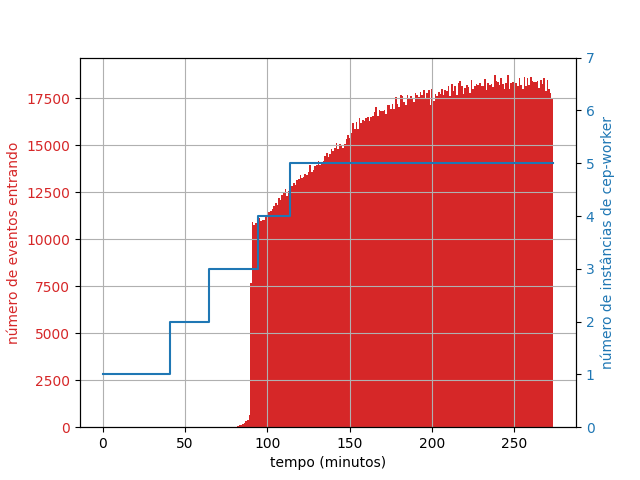
\includegraphics[width=\textwidth]{figuras/graphics/carga_e_workers_total7-dez-is.png}
\caption{Número de eventos entrando no sistema (em vermelho) e número de instâncias de \texttt{CEP Worker} (em azul) em função do tempo na execução 2 do experimento utilizando o algoritmo de balanceamento de carga por Similaridade de Entrada.}
\label{fig:workers_and_load_total-7-dez-is}
\end{subfigure}%

\begin{subfigure}{\textwidth}
\centering
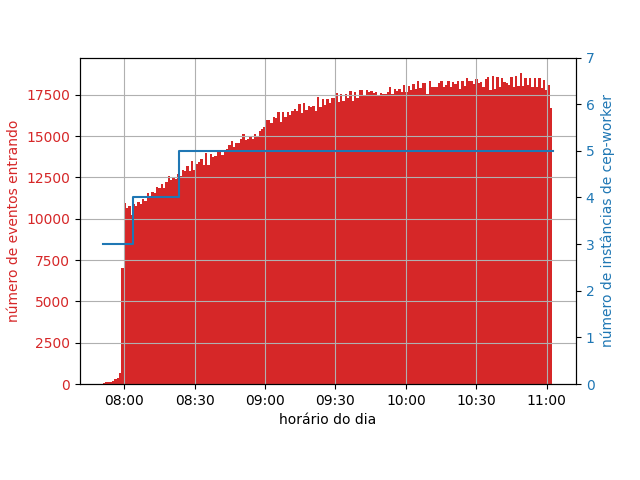
\includegraphics[width=\textwidth]{figuras/graphics/carga_e_workers_horario7-dez-is.png}
\caption{Número de eventos entrando no sistema (em vermelho) e número de instâncias de \texttt{CEP Worker} (em azul) em função do horário do dia na execução 2 do experimento utilizando o algoritmo de balanceamento de carga por Similaridade de Entrada.}
\label{fig:workers_and_load_SPtrans-7-dez-is}
\end{subfigure}%
\caption{Número de eventos entrando no sistema e número de instâncias de \texttt{CEP Worker} na execução 2 do experimento utilizando o algoritmo de balanceamento de carga por Similaridade de Entrada.}
\end{figure}






%\subsection{Latência}


\begin{figure}
\centering
\begin{subfigure}{.5\textwidth}
\centering
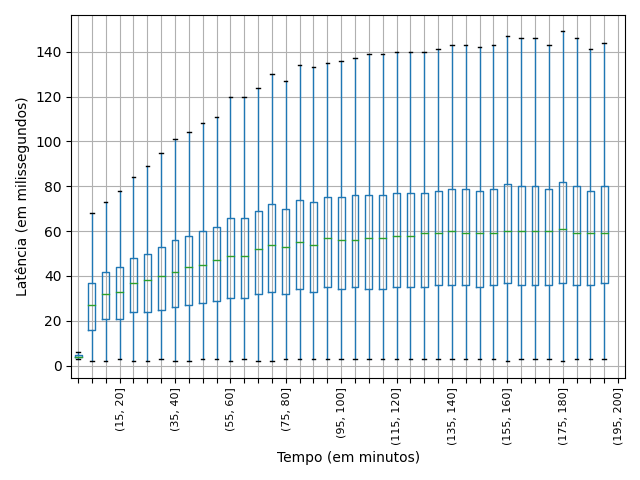
\includegraphics[width=\textwidth]{figuras/graphics/boxplot_7-dez-is_vf.png}
\caption{BoxPlot da latência da categoria de tipos de evento \textbf{vf} por intervalos de cinco minutos ao longo da execução  2 do experimento utilizando o algoritmo de balanceamento de carga por Similaridade de Entrada.}
\label{fig:BoxPlot_vf_7-dez-is}
\end{subfigure}%
%\end{figure}

%\begin{figure}
\begin{subfigure}{.5\textwidth}
\centering
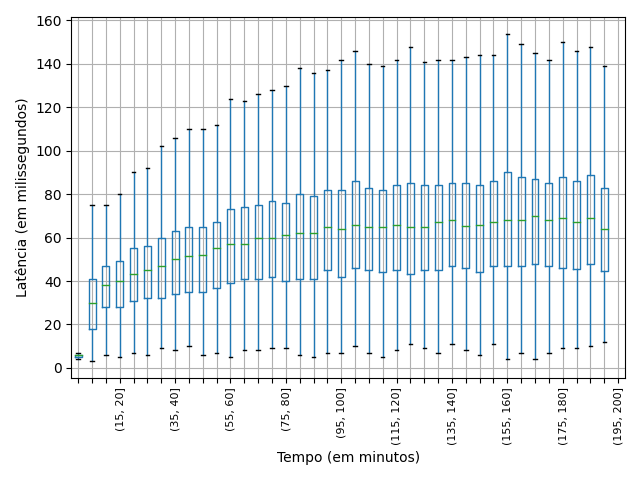
\includegraphics[width=\textwidth]{figuras/graphics/boxplot_7-dez-is_vi.png}
\caption{BoxPlot da latência da categoria de tipos de evento \textbf{vi} por intervalos de cinco minutos ao longo da execução 2 do experimento utilizando o algoritmo de balanceamento de carga por Similaridade de Entrada.}
\label{fig:BoxPlot_vi_IS_7-dez-is}
\end{subfigure}%
%\end{figure}
\centering
%\begin{figure}
\begin{subfigure}{.5\textwidth}
\centering
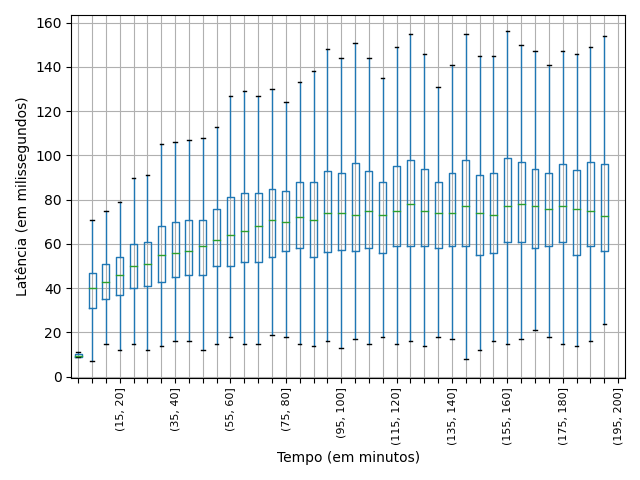
\includegraphics[width=\textwidth]{figuras/graphics/boxplot_7-dez-is_vel.png}
\caption{BoxPlot da latência da categoria de tipos de evento \textbf{vel} por intervalos de cinco minutos ao longo da execução 2 do experimento utilizando o algoritmo de balanceamento de carga por Similaridade de Entrada.}
\label{fig:BoxPlot_vel_IS_7-dez-is}
\end{subfigure}%
%\end{figure}

%\begin{figure}
\begin{subfigure}{.5\textwidth}
\centering
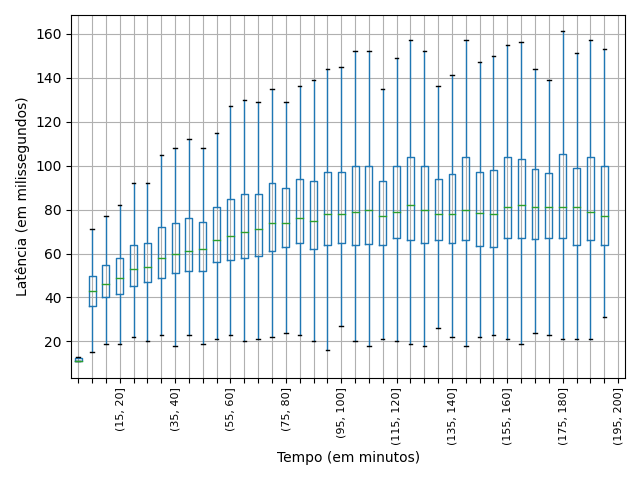
\includegraphics[width=\textwidth]{figuras/graphics/boxplot_7-dez-is_corr.png}
\caption{BoxPlot da latência da categoria de tipos de evento \textbf{corr} por intervalos de cinco minutos ao longo da execução 2 do experimento utilizando o algoritmo de balanceamento de carga por Similaridade de Entrada.}
\label{fig:BoxPlot_corr_IS_7-dez-is}
\end{subfigure}%
%\end{figure}
%\begin{figure}
\begin{subfigure}{.5\textwidth}
\centering
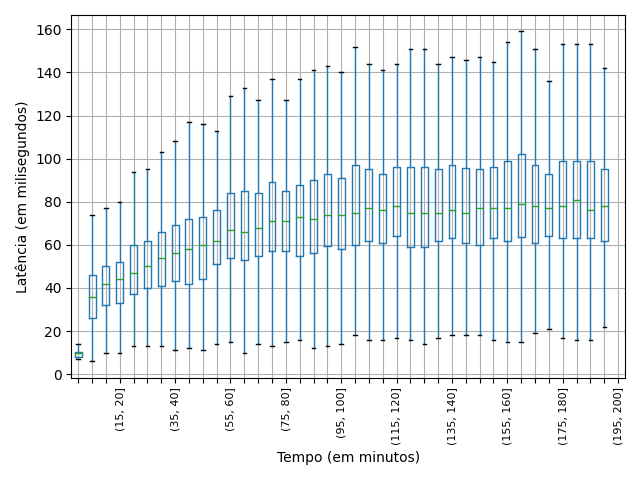
\includegraphics[width=\textwidth]{figuras/graphics/boxplot_7-dez-is_busb.png}
\caption{BoxPlot da latência da categoria de tipos de evento \textbf{BusB} por intervalos de cinco minutos ao longo da execução 2 do experimento utilizando o algoritmo de balanceamento de carga por Similaridade de Entrada.}
\label{fig:BoxPlot_BusB_IS_7-dez-is}
\end{subfigure}%
\caption{BoxPlot da latência por intervalos de cinco minutos ao longo da execução 2 do experimento utilizando o algoritmo de balanceamento de carga por Similaridade de Entrada.}
\end{figure}


%\newpage

%----------------------------------------------------------------


%\section{Experimento 3 - Algoritmo de Uso de Estado}

%\subsection{Vazão}


\begin{figure}[h]
\centering
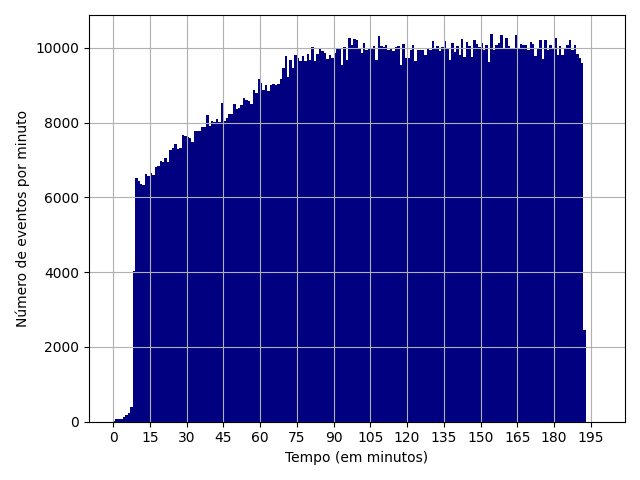
\includegraphics[width=\textwidth]{figuras/graphics/histogram_vazao_8-dez-su.png}
\caption{Vazão de eventos detectados pelo sistema na execução 3 do experimento utilizando o algoritmo de balanceamento por Uso de Estado.}
\label{fig:vazao_8-dez-su}
\end{figure}

%\subsection{Número de instâncias e de eventos de entrada}


\begin{figure}[h]
\centering
\begin{subfigure}{0.9\textwidth}
\centering
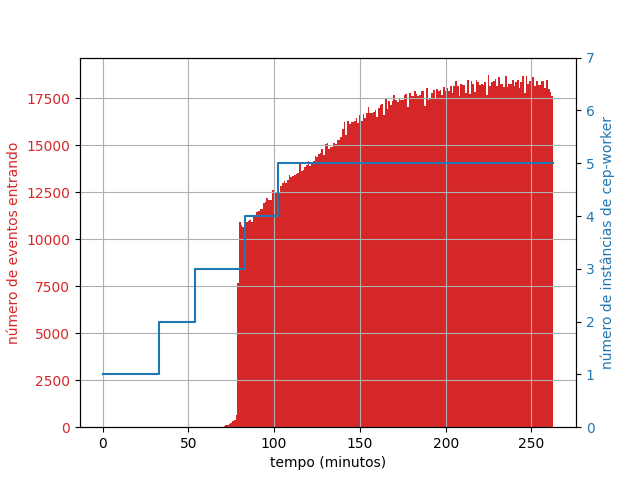
\includegraphics[width=\textwidth]{figuras/graphics/carga_e_workers_total8-dez-su.png}
\caption{Número de eventos entrando no sistema (em vermelho) e número de instâncias de \texttt{CEP Worker} (em azul) em função do tempo na execução 3 do experimento utilizando o algoritmo de balanceamento de carga por Uso de Estado.}
\label{fig:workers_and_load_total_8-dez-su}
\end{subfigure}%

\begin{subfigure}{\textwidth}
\centering
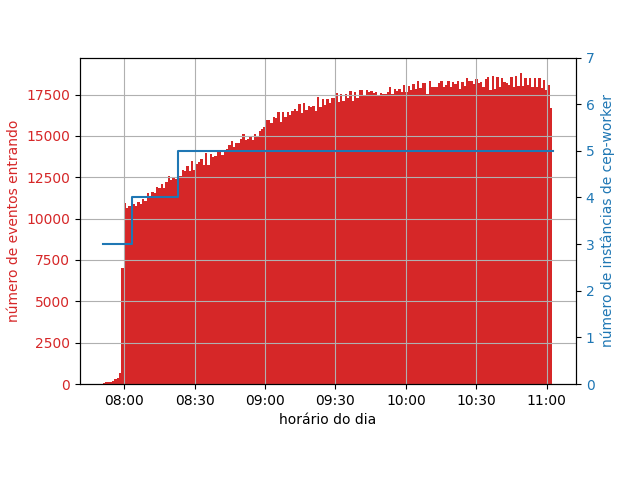
\includegraphics[width=\textwidth]{figuras/graphics/carga_e_workers_horario8-dez-su.png}
\caption{Número de eventos entrando no sistema (em vermelho) e número de instâncias de \texttt{CEP Worker} (em azul) em função do horário do dia na execução 3 do experimento utilizando o algoritmo de balanceamento de carga por Uso de Estado.}
\label{fig:workers_and_load_SPtrans_8-dez-su}
\end{subfigure}%
\caption{Número de eventos entrando no sistema e número de instâncias de \texttt{CEP Worker} na execução 3 do experimento utilizando o algoritmo de balanceamento de carga por Uso de Estado.}
\end{figure}

%\subsection{Latência}


\begin{figure}
\centering
\begin{subfigure}{.5\textwidth}
\centering
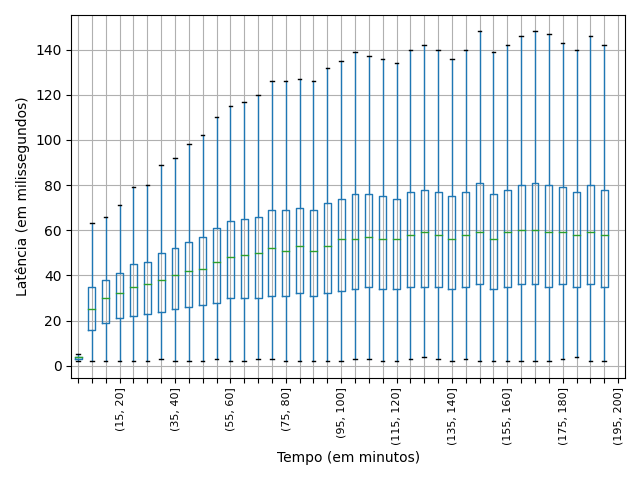
\includegraphics[width=\textwidth]{figuras/graphics/boxplot_8-dez-su_vf.png}
\caption{BoxPlot da latência da categoria de tipos de evento \textbf{vf} por intervalos de cinco minutos ao longo da execução 3 do experimento utilizando o algoritmo de balanceamento de carga por Uso de Estado.}
\label{fig:BoxPlot_vf_SU_8-dez-su}
\end{subfigure}%
%\end{figure}

%\begin{figure}
\begin{subfigure}{.5\textwidth}
\centering
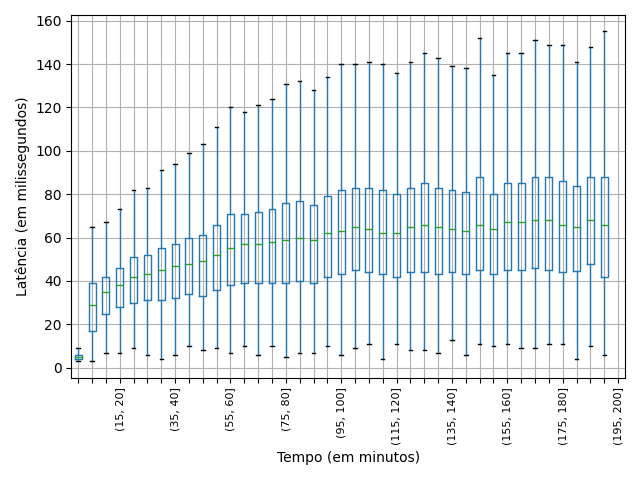
\includegraphics[width=\textwidth]{figuras/graphics/boxplot_8-dez-su_vi.png}
\caption{BoxPlot da latência da categoria de tipos de evento \textbf{vi} por intervalos de cinco minutos ao longo da execução 3 do experimento utilizando o algoritmo de balanceamento de carga por Uso de Estado.}
\label{fig:BoxPlot_vi_SU_8-dez-su}
\end{subfigure}%
%\end{figure}
\centering
%\begin{figure}
\begin{subfigure}{.5\textwidth}
\centering
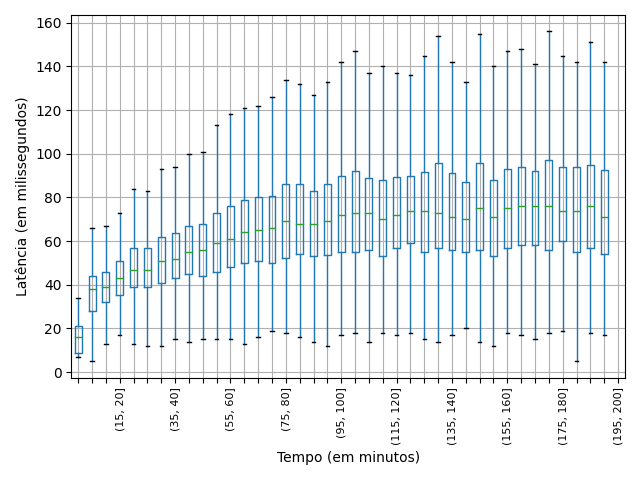
\includegraphics[width=\textwidth]{figuras/graphics/boxplot_8-dez-su_vel.png}
\caption{BoxPlot da latência da categoria de tipos de evento \textbf{vel} por intervalos de cinco minutos ao longo da execução 3 do experimento utilizando o algoritmo de balanceamento de carga por Uso de Estado.}
\label{fig:BoxPlot_vel_SU_8-dez-su}
\end{subfigure}%
%\end{figure}

%\begin{figure}
\begin{subfigure}{.5\textwidth}
\centering
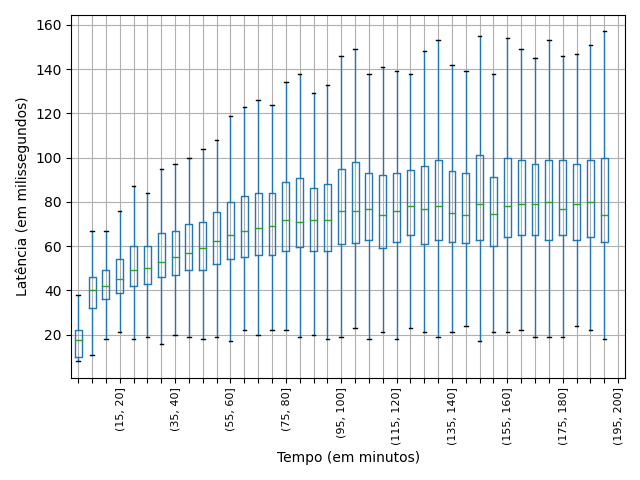
\includegraphics[width=\textwidth]{figuras/graphics/boxplot_8-dez-su_corr.png}
\caption{BoxPlot da latência da categoria de tipos de evento \textbf{corr} por intervalos de cinco minutos ao longo da execução 3 do experimento utilizando o algoritmo de balanceamento de carga por Uso de Estado.}
\label{fig:BoxPlot_corr_SU_8-dez-su}
\end{subfigure}%
%\end{figure}
%\begin{figure}
\begin{subfigure}{.5\textwidth}
\centering
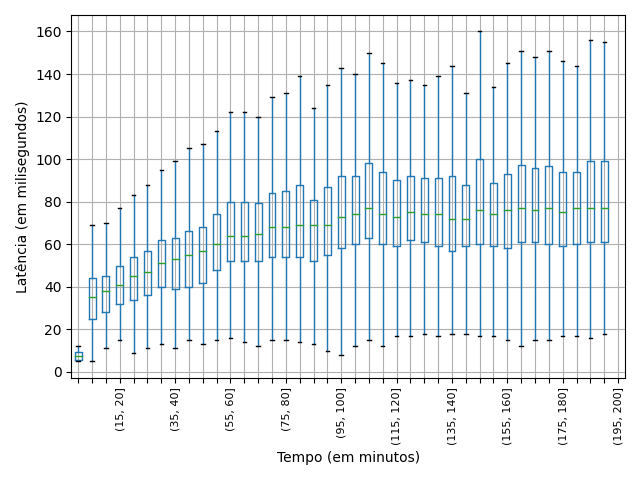
\includegraphics[width=\textwidth]{figuras/graphics/boxplot_8-dez-su_busb.png}
\caption{BoxPlot da latência da categoria de tipos de evento \textbf{BusB} por intervalos de cinco minutos ao longo da execução 3 do experimento utilizando o algoritmo de balanceamento de carga por Uso de Estado.}
\label{fig:BoxPlot_BusB_SU_8-dez-su}
\end{subfigure}%
\caption{BoxPlot da latência por intervalos de cinco minutos ao longo da execução 3 do experimento utilizando o algoritmo de balanceamento de carga por Uso de Estado.}
\end{figure}






%----------------------------------------
%\newpage
%\section{Experimento 3 - Algoritmo de Similaridade de Entrada}

%\subsection{Vazão}


\begin{figure}[h]
\centering
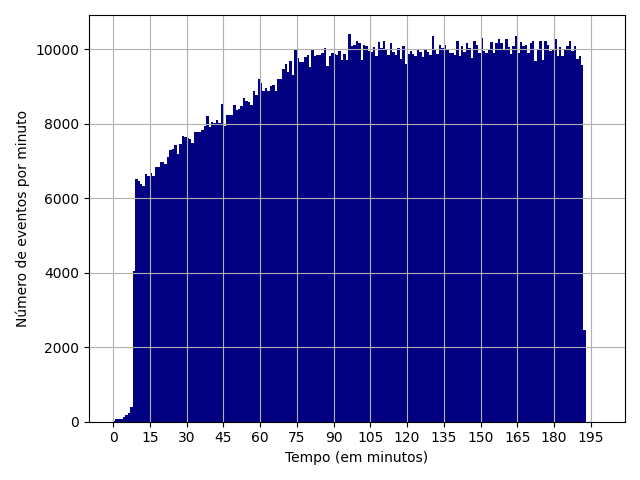
\includegraphics[width=\textwidth]{figuras/graphics/histogram_vazao_8-dez-is.png}
\caption{Vazão de eventos detectados pelo sistema na execução 3 do experimento utilizando o algoritmo de balanceamento por Similaridade de Entrada.}
\label{fig:vazao_8-dez-is}
\end{figure}

%\subsection{Número de instâncias e de eventos de entrada}


\begin{figure}[h]
\centering
\begin{subfigure}{0.9\textwidth}
\centering
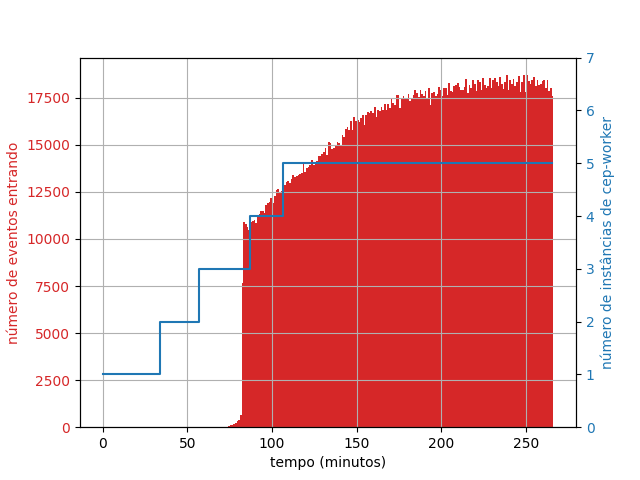
\includegraphics[width=\textwidth]{figuras/graphics/carga_e_workers_total8-dez-is.png}
\caption{Número de eventos entrando no sistema (em vermelho) e número de instâncias de \texttt{CEP Worker} (em azul) em função do tempo na execução 3 do experimento utilizando o algoritmo de balanceamento de carga por Similaridade de Entrada.}
\label{fig:workers_and_load_total-8-dez-is}
\end{subfigure}%

\begin{subfigure}{\textwidth}
\centering
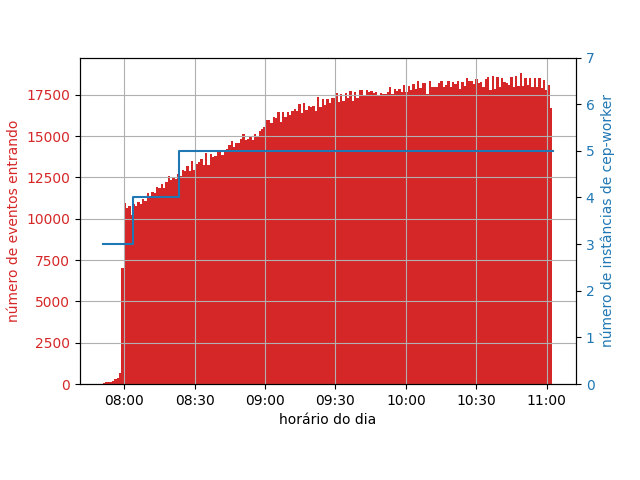
\includegraphics[width=\textwidth]{figuras/graphics/carga_e_workers_horario8-dez-is.png}
\caption{Número de eventos entrando no sistema (em vermelho) e número de instâncias de \texttt{CEP Worker} (em azul) em função do horário do dia na execução 3 do experimento utilizando o algoritmo de balanceamento de carga por Similaridade de Entrada.}
\label{fig:workers_and_load_SPtrans-8-dez-is}
\end{subfigure}%
\caption{Número de eventos entrando no sistema e número de instâncias de \texttt{CEP Worker} na execução 3 do experimento utilizando o algoritmo de balanceamento de carga por Similaridade de Entrada.}
\end{figure}




%\subsection{Latência}


\begin{figure}
\centering
\begin{subfigure}{.5\textwidth}
\centering
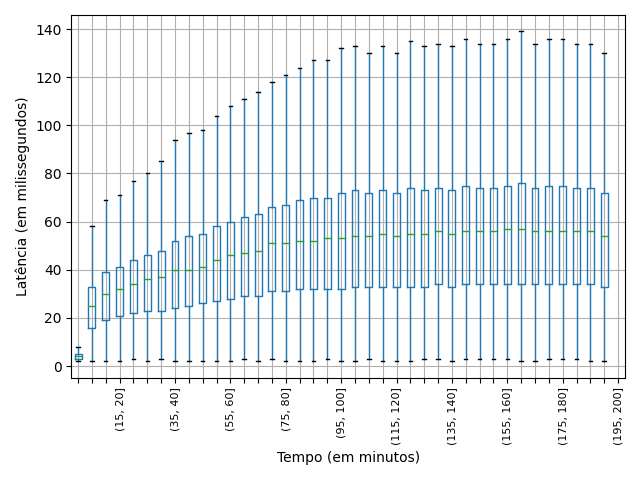
\includegraphics[width=\textwidth]{figuras/graphics/boxplot_8-dez-is_vf.png}
\caption{BoxPlot da latência da categoria de tipos de evento \textbf{vf} por intervalos de cinco minutos ao longo da execução 3 do experimento utilizando o algoritmo de balanceamento por Similaridade de Entrada.}
\label{fig:BoxPlot_vf_8-dez-is}
\end{subfigure}%
%\end{figure}

%\begin{figure}
\begin{subfigure}{.5\textwidth}
\centering
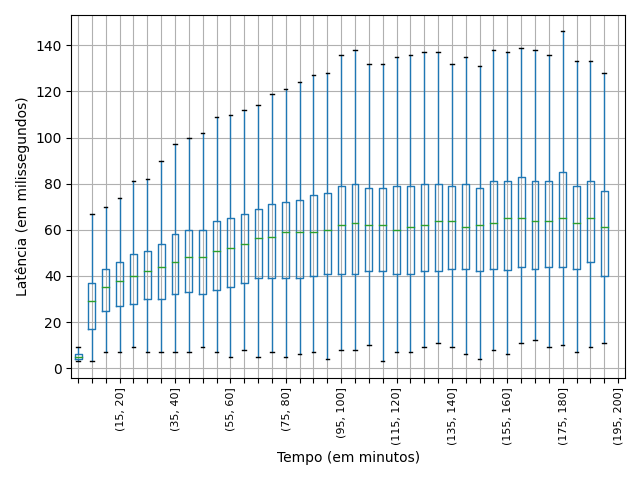
\includegraphics[width=\textwidth]{figuras/graphics/boxplot_8-dez-is_vi.png}
\caption{BoxPlot da latência da categoria de tipos de evento \textbf{vi} por intervalos de cinco minutos ao longo da execução 3 do experimento utilizando o algoritmo de balanceamento por Similaridade de Entrada.}
\label{fig:BoxPlot_vi_IS_8-dez-is}
\end{subfigure}%
%\end{figure}
\centering
%\begin{figure}
\begin{subfigure}{.5\textwidth}
\centering
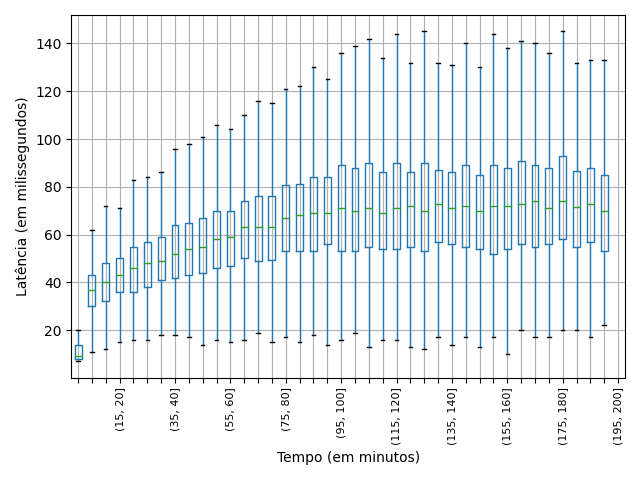
\includegraphics[width=\textwidth]{figuras/graphics/boxplot_8-dez-is_vel.png}
\caption{BoxPlot da latência da categoria de tipos de evento \textbf{vel} por intervalos de cinco minutos ao longo da execução 3 do experimento utilizando o algoritmo de balanceamento por Similaridade de Entrada.}
\label{fig:BoxPlot_vel_IS_8-dez-is}
\end{subfigure}%
%\end{figure}

%\begin{figure}
\begin{subfigure}{.5\textwidth}
\centering
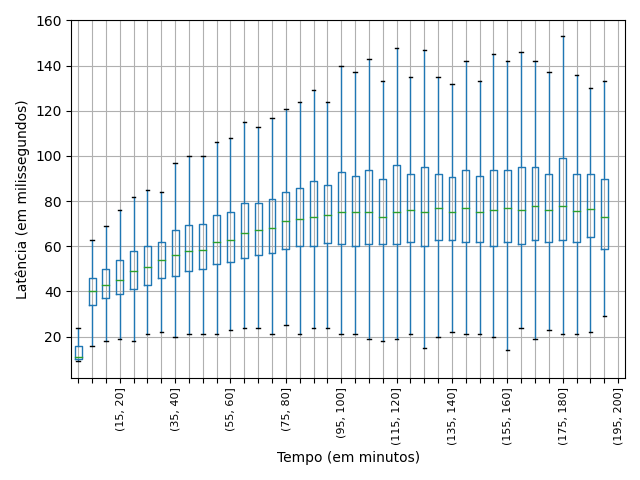
\includegraphics[width=\textwidth]{figuras/graphics/boxplot_8-dez-is_corr.png}
\caption{BoxPlot da latência da categoria de tipos de evento \textbf{corr} por intervalos de cinco minutos ao longo da execução 3 do experimento utilizando o algoritmo de balanceamento por Similaridade de Entrada.}
\label{fig:BoxPlot_corr_IS_8-dez-is}
\end{subfigure}%
%\end{figure}
%\begin{figure}
\begin{subfigure}{.5\textwidth}
\centering
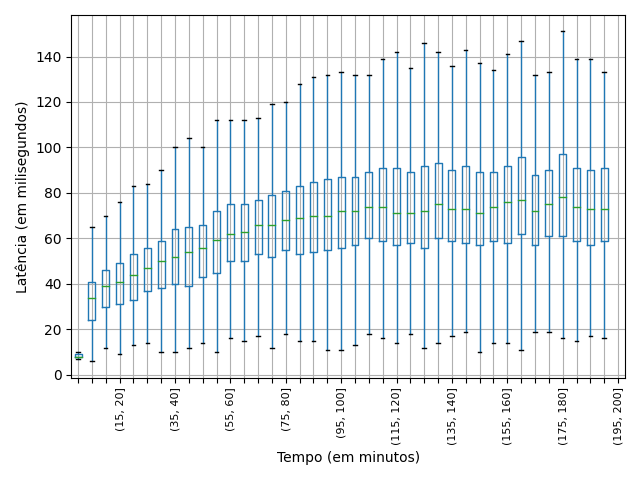
\includegraphics[width=\textwidth]{figuras/graphics/boxplot_8-dez-is_busb.png}
\caption{BoxPlot da latência da categoria de tipos de evento \textbf{BusB} por intervalos de cinco minutos ao longo da execução 3 do experimento utilizando o algoritmo de balanceamento por Similaridade de Entrada.}
\label{fig:BoxPlot_BusB_IS_8-dez-is}
\end{subfigure}%
\caption{BoxPlot da latência por intervalos de cinco minutos ao longo da execução 3 do experimento utilizando o algoritmo de balanceamento de carga por Similaridade de Entrada.}
\end{figure}



%\newpage

%------------------------------------------------------------



%\section{Experimento 4 - Algoritmo de Uso de Estado}

%\subsection{Vazão}


\begin{figure}[h]
\centering
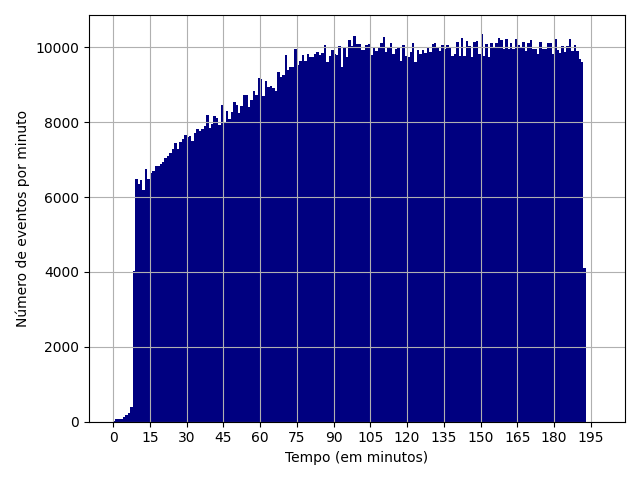
\includegraphics[width=\textwidth]{figuras/graphics/histogram_vazao_9-dez-su.png}
\caption{Vazão de eventos detectados pelo sistema na execução 4 do experimento utilizando o algoritmo de balanceamento por Uso de Estado.}
\label{fig:vazao_9-dez-su}
\end{figure}

%\subsection{Número de instâncias e de eventos de entrada}


\begin{figure}[h]
\centering
\begin{subfigure}{0.9\textwidth}
\centering
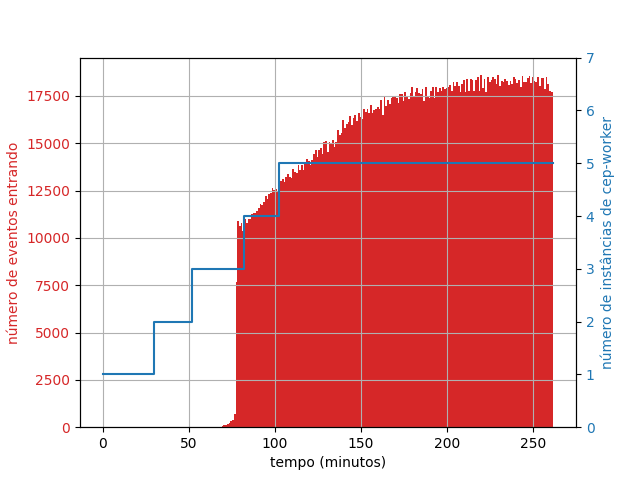
\includegraphics[width=\textwidth]{figuras/graphics/carga_e_workers_total9-dez-su.png}
\caption{Número de eventos entrando no sistema (em vermelho) e número de instâncias de \texttt{CEP Worker} (em azul) em função do tempo na execução 4 do experimento utilizando o algoritmo de balanceamento de carga por Uso de Estado.}
\label{fig:workers_and_load_total_9-dez-su}
\end{subfigure}%

\begin{subfigure}{\textwidth}
\centering
\includegraphics[width=\textwidth]{figuras/graphics/carga_e_workers_horario9-dez-su.png}
\caption{Número de eventos entrando no sistema (em vermelho) e número de instâncias de \texttt{CEP Worker} (em azul) em função do horário do dia na execução 4 do experimento utilizando o algoritmo de balanceamento de carga por Uso de Estado.}
\label{fig:workers_and_load_SPtrans_9-dez-su}
\end{subfigure}%
\caption{Número de eventos entrando no sistema e número de instâncias de \texttt{CEP Worker} na execução 4 do experimento utilizando o algoritmo de balanceamento de carga por Uso de Estado.}
\end{figure}

%\subsection{Latência}


\begin{figure}
\centering
\begin{subfigure}{.5\textwidth}
\centering
\includegraphics[width=\textwidth]{figuras/graphics/boxplot_9-dez-su_vf.png}
\caption{BoxPlot da latência da categoria de tipos de evento \textbf{vf} por intervalos de cinco minutos ao longo da execução 4 do experimento utilizando o algoritmo de balanceamento de carga por Uso de Estado.}
\label{fig:BoxPlot_vf_SU_9-dez-su}
\end{subfigure}%
%\end{figure}

%\begin{figure}
\begin{subfigure}{.5\textwidth}
\centering
\includegraphics[width=\textwidth]{figuras/graphics/boxplot_9-dez-su_vi.png}
\caption{BoxPlot da latência da categoria de tipos de evento \textbf{vi} por intervalos de cinco minutos ao longo da execução 4 do experimento utilizando o algoritmo de balanceamento de carga por Uso de Estado.}
\label{fig:BoxPlot_vi_SU_9-dez-su}
\end{subfigure}%
%\end{figure}
\centering
%\begin{figure}
\begin{subfigure}{.5\textwidth}
\centering
\includegraphics[width=\textwidth]{figuras/graphics/boxplot_9-dez-su_vel.png}
\caption{BoxPlot da latência da categoria de tipos de evento \textbf{vel} por intervalos de cinco minutos ao longo da execução 4 do experimento utilizando o algoritmo de balanceamento de carga por Uso de Estado.}
\label{fig:BoxPlot_vel_SU_9-dez-su}
\end{subfigure}%
%\end{figure}

%\begin{figure}
\begin{subfigure}{.5\textwidth}
\centering
\includegraphics[width=\textwidth]{figuras/graphics/boxplot_9-dez-su_corr.png}
\caption{BoxPlot da latência da categoria de tipos de evento \textbf{corr} por intervalos de cinco minutos ao longo da execução 4 do experimento utilizando o algoritmo de balanceamento de carga por Uso de Estado.}
\label{fig:BoxPlot_corr_SU_9-dez-su}
\end{subfigure}%
%\end{figure}
%\begin{figure}
\begin{subfigure}{.5\textwidth}
\centering
\includegraphics[width=\textwidth]{figuras/graphics/boxplot_9-dez-su_busb.png}
\caption{BoxPlot da latência da categoria de tipos de evento \textbf{BusB} por intervalos de cinco minutos ao longo da execução 4 do experimento utilizando o algoritmo de balanceamento de carga por Uso de Estado.}
\label{fig:BoxPlot_BusB_SU_9-dez-su}
\end{subfigure}%
\caption{BoxPlot da latência por intervalos de cinco minutos ao longo da execução 4 do experimento utilizando o algoritmo de balanceamento de carga por Uso de Estado.}
\end{figure}






%----------------------------------------
%\newpage
%\section{Experimento 4 - Algoritmo de Similaridade de Entrada}

%\subsection{Vazão}


\begin{figure}[h]
\centering
\includegraphics[width=\textwidth]{figuras/graphics/histogram_vazao_9-dez-is.png}
\caption{Vazão de eventos detectados pelo sistema na execução 4 do experimento utilizando o algoritmo de balanceamento por Similaridade de Entrada.}
\label{fig:vazao_9-dez-is}
\end{figure}

%\subsection{Número de instâncias e de eventos de entrada}


\begin{figure}[h]
\centering
\begin{subfigure}{0.9\textwidth}
\centering
\includegraphics[width=\textwidth]{figuras/graphics/carga_e_workers_total9-dez-is.png}
\caption{Número de eventos entrando no sistema (em vermelho) e número de instâncias de \texttt{CEP Worker} (em azul) em função do tempo na execução 4 do experimento utilizando o algoritmo de balanceamento de carga por Similaridade de Entrada.}
\label{fig:workers_and_load_total-9-dez-is}
\end{subfigure}%

\begin{subfigure}{\textwidth}
\centering
\includegraphics[width=\textwidth]{figuras/graphics/carga_e_workers_horario9-dez-is.png}
\caption{Número de eventos entrando no sistema (em vermelho) e número de instâncias de \texttt{CEP Worker} (em azul) em função do horário do dia na execução 4 do experimento utilizando o algoritmo de balanceamento de carga por Similaridade de Entrada.}
\label{fig:workers_and_load_SPtrans-9-dez-is}
\end{subfigure}%
\caption{Número de eventos entrando no sistema e número de instâncias de \texttt{CEP Worker} na execução 5 do experimento utilizando o algoritmo de balanceamento de carga por Similaridade de Entrada.}
\end{figure}






%\subsection{Latência}


\begin{figure}
\centering
\begin{subfigure}{.5\textwidth}
\centering
\includegraphics[width=\textwidth]{figuras/graphics/boxplot_9-dez-is_vf.png}
\caption{BoxPlot da latência da categoria de tipos de evento \textbf{vf} por intervalos de cinco minutos ao longo da execução 4 do experimento utilizando o algoritmo de balanceamento de carga por Similaridade de Entrada.}
\label{fig:BoxPlot_vf_9-dez-is}
\end{subfigure}%
%\end{figure}

%\begin{figure}
\begin{subfigure}{.5\textwidth}
\centering
\includegraphics[width=\textwidth]{figuras/graphics/boxplot_9-dez-is_vi.png}
\caption{BoxPlot da latência da categoria de tipos de evento \textbf{vi} por intervalos de cinco minutos ao longo da execução 4 do experimento utilizando o algoritmo de balanceamento de carga por Similaridade de Entrada.}
\label{fig:BoxPlot_vi_IS_9-dez-is}
\end{subfigure}%
%\end{figure}
\centering
%\begin{figure}
\begin{subfigure}{.5\textwidth}
\centering
\includegraphics[width=\textwidth]{figuras/graphics/boxplot_9-dez-is_vel.png}
\caption{BoxPlot da latência da categoria de tipos de evento \textbf{vel} por intervalos de cinco minutos ao longo da execução 4 do experimento utilizando o algoritmo de balanceamento de carga por Similaridade de Entrada.}
\label{fig:BoxPlot_vel_IS_9-dez-is}
\end{subfigure}%
%\end{figure}

%\begin{figure}
\begin{subfigure}{.5\textwidth}
\centering
\includegraphics[width=\textwidth]{figuras/graphics/boxplot_9-dez-is_corr.png}
\caption{BoxPlot da latência da categoria de tipos de evento \textbf{corr} por intervalos de cinco minutos ao longo da execução 4 do experimento utilizando o algoritmo de balanceamento de carga por Similaridade de Entrada.}
\label{fig:BoxPlot_corr_IS_9-dez-is}
\end{subfigure}%
%\end{figure}
%\begin{figure}
\begin{subfigure}{.5\textwidth}
\centering
\includegraphics[width=\textwidth]{figuras/graphics/boxplot_9-dez-is_busb.png}
\caption{BoxPlot da latência da categoria de tipos de evento \textbf{BusB} por intervalos de cinco minutos ao longo da execução 4 do experimento utilizando o algoritmo de balanceamento de carga por Similaridade de Entrada.}
\label{fig:BoxPlot_BusB_IS_9-dez-is}
\end{subfigure}%
\caption{BoxPlot da latência por intervalos de cinco minutos ao longo da execução 4 do experimento utilizando o algoritmo de balanceamento de carga por Similaridade de Entrada.}
\end{figure}



%--------777777777777777777777777777777777777
%\newpage

%\section{Experimento 5 - Algoritmo de Uso de Estado}

%\subsection{Vazão}


\begin{figure}[h]
\centering
\includegraphics[width=\textwidth]{figuras/graphics/histogram_vazao_10-dez-su.png}
\caption{Vazão de eventos detectados pelo sistema na execução 5 do experimento utilizando o algoritmo de balanceamento por Uso de Estado.}
\label{fig:vazao_9-dez-su}
\end{figure}



%\subsection{Número de instâncias e de eventos de entrada}


\begin{figure}[h]
\centering
\begin{subfigure}{\textwidth}
\centering
\includegraphics[width=0.9\textwidth]{figuras/graphics/carga_e_workers_total10-dez-su.png}
\caption{Número de eventos entrando no sistema (em vermelho) e número de instâncias de \texttt{CEP Worker} (em azul) em função do tempo na execução 5 do experimento utilizando o algoritmo de balanceamento de carga por Uso de Estado.}
\label{fig:workers_and_load_total_10-dez-su}
\end{subfigure}%

\begin{subfigure}{\textwidth}
\centering
\includegraphics[width=\textwidth]{figuras/graphics/carga_e_workers_horario10-dez-su.png}
\caption{Número de eventos entrando no sistema (em vermelho) e número de instâncias de \texttt{CEP Worker} (em azul) em função do horário do dia na execução 5 do experimento utilizando o algoritmo de balanceamento de carga por Uso de Estado.}
\label{fig:workers_and_load_SPtrans_10-dez-su}
\end{subfigure}%
\caption{Número de eventos entrando no sistema e número de instâncias de \texttt{CEP Worker} na execução 5 do experimento utilizando o algoritmo de balanceamento de carga por Uso de Estado.}
\end{figure}



%\subsection{Latência}


\begin{figure}
\centering
\begin{subfigure}{.5\textwidth}
\centering
\includegraphics[width=\textwidth]{figuras/graphics/boxplot_10-dez-su_vf.png}
\caption{BoxPlot da latência da categoria de tipos de evento \textbf{vf} por intervalos de cinco minutos ao longo da execução 5 do experimento utilizando o algoritmo de balanceamento de carga por Uso de Estado.}
\label{fig:BoxPlot_vf_SU_10-dez-su}
\end{subfigure}%
%\end{figure}

%\begin{figure}
\begin{subfigure}{.5\textwidth}
\centering
\includegraphics[width=\textwidth]{figuras/graphics/boxplot_10-dez-su_vi.png}
\caption{BoxPlot da latência da categoria de tipos de evento \textbf{vi} por intervalos de cinco minutos ao longo da execução 5 do experimento utilizando o algoritmo de balanceamento de carga por Uso de Estado.}
\label{fig:BoxPlot_vi_SU_10-dez-su}
\end{subfigure}%
%\end{figure}
\centering
%\begin{figure}
\begin{subfigure}{.5\textwidth}
\centering
\includegraphics[width=\textwidth]{figuras/graphics/boxplot_10-dez-su_vel.png}
\caption{BoxPlot da latência da categoria de tipos de evento \textbf{vel} por intervalos de cinco minutos ao longo da execução 5 do experimento utilizando o algoritmo de balanceamento de carga por Uso de Estado.}
\label{fig:BoxPlot_vel_SU_10-dez-su}
\end{subfigure}%
%\end{figure}

%\begin{figure}
\begin{subfigure}{.5\textwidth}
\centering
\includegraphics[width=\textwidth]{figuras/graphics/boxplot_10-dez-su_corr.png}
\caption{BoxPlot da latência da categoria de tipos de evento \textbf{corr} por intervalos de cinco minutos ao longo da execução 5 do experimento utilizando o algoritmo de balanceamento de carga por Uso de Estado.}
\label{fig:BoxPlot_corr_SU_10-dez-su}
\end{subfigure}%
%\end{figure}
%\begin{figure}
\begin{subfigure}{.5\textwidth}
\centering
\includegraphics[width=\textwidth]{figuras/graphics/boxplot_10-dez-su_busb.png}
\caption{BoxPlot da latência da categoria de tipos de evento \textbf{BusB} por intervalos de cinco minutos ao longo da execução 5 do experimento utilizando o algoritmo de balanceamento de carga por Uso de Estado.}
\label{fig:BoxPlot_BusB_SU_10-dez-su}
\end{subfigure}%
\caption{BoxPlot da latência por intervalos de cinco minutos ao longo da execução 5 do experimento utilizando o algoritmo de balanceamento de carga por Uso de Estado.}
\end{figure}




%----------------------------------------
%\newpage
%\section{Experimento 5 - Algoritmo de Similaridade de Entrada}

%\subsection{Vazão}


\begin{figure}[h]
\centering
\includegraphics[width=\textwidth]{figuras/graphics/histogram_vazao_10-dez-is.png}
\caption{Vazão de eventos detectados pelo sistema na execução 5 do experimento utilizando o algoritmo de balanceamento por Similaridade de Entrada.}
\label{fig:vazao_10-dez-is}
\end{figure}

%\subsection{Número de instâncias e de eventos de entrada}


\begin{figure}[h]
\begin{subfigure}{0.9\textwidth}
\includegraphics[width=\textwidth]{figuras/graphics/carga_e_workers_total10-dez-is.png}
\caption{Número de eventos entrando no sistema (em vermelho) e número de instâncias de \texttt{CEP Worker} (em azul) em função do tempo na execução 5 do experimento utilizando o algoritmo de balanceamento de carga por Similaridade de Entrada.}
\label{fig:workers_and_load_total-10-dez-is}
\end{subfigure}

\begin{subfigure}{\textwidth}
\includegraphics[width=\textwidth]{figuras/graphics/carga_e_workers_horario10-dez-is.png}
\caption{Número de eventos entrando no sistema (em vermelho) e número de instâncias de \texttt{CEP Worker} (em azul) em função do horário do dia na execução 5 do experimento utilizando o algoritmo de balanceamento de carga por Similaridade de Entrada.}
\label{fig:workers_and_load_SPtrans-10-dez-is}
\end{subfigure}%
\end{figure}



%\subsection{Latência}


\begin{figure}
\centering
\begin{subfigure}{.5\textwidth}
\centering
\includegraphics[width=\textwidth]{figuras/graphics/boxplot_10-dez-is_vf.png}
\caption{BoxPlot da latência da categoria de tipos de evento \textbf{vf} por intervalos de cinco minutos ao longo da execução 5 do experimento utilizando o algoritmo de balanceamento de carga por Similaridade de Entrada.}
\label{fig:BoxPlot_vf_10-dez-is}
\end{subfigure}%
%\end{figure}

%\begin{figure}
\begin{subfigure}{.5\textwidth}
\centering
\includegraphics[width=\textwidth]{figuras/graphics/boxplot_10-dez-is_vi.png}
\caption{BoxPlot da latência da categoria de tipos de evento \textbf{vi} por intervalos de cinco minutos ao longo da execução 5 do experimento utilizando o algoritmo de balanceamento de carga por Similaridade de Entrada.}
\label{fig:BoxPlot_vi_IS_10-dez-is}
\end{subfigure}%
%\end{figure}
\centering
%\begin{figure}
\begin{subfigure}{.5\textwidth}
\centering
\includegraphics[width=\textwidth]{figuras/graphics/boxplot_10-dez-is_vel.png}
\caption{BoxPlot da latência da categoria de tipos de evento \textbf{vel} por intervalos de cinco minutos ao longo da execução 5 do experimento utilizando o algoritmo de balanceamento de carga por Similaridade de Entrada.}
\label{fig:BoxPlot_vel_IS_10-dez-is}
\end{subfigure}%
%\end{figure}

%\begin{figure}
\begin{subfigure}{.5\textwidth}
\centering
\includegraphics[width=\textwidth]{figuras/graphics/boxplot_10-dez-is_corr.png}
\caption{BoxPlot da latência da categoria de tipos de evento \textbf{corr} por intervalos de cinco minutos ao longo da execução 5 do experimento utilizando o algoritmo de balanceamento de carga por Similaridade de Entrada.}
\label{fig:BoxPlot_corr_IS_10-dez-is}
\end{subfigure}%
%\end{figure}
%\begin{figure}
\begin{subfigure}{.5\textwidth}
\centering
\includegraphics[width=\textwidth]{figuras/graphics/boxplot_10-dez-is_busb.png}
\caption{BoxPlot da latência da categoria de tipos de evento \textbf{BusB} por intervalos de cinco minutos ao longo da execução 5 do experimento utilizando o algoritmo de balanceamento de carga por Similaridade de Entrada.}
\label{fig:BoxPlot_BusB_IS_10-dez-is}
\end{subfigure}%
\caption{BoxPlot da latência por intervalos de cinco minutos ao longo da execução 5 do experimento utilizando o algoritmo de balanceamento de carga por Similaridade de Entrada.}
\end{figure}




%\section{Velocidade média ao longo do horário nos corredores de ônibus}
\newpage

%\section{Velocidade média de cada corredor pelo horário da SPTrans}

\begin{figure}[ht]
\centering
\begin{subfigure}{.45\textwidth}
  \centering
  \includegraphics[width=\textwidth]{figuras/detect_graphics/avg_speed_7-dez-su-corr_Ibirapuera.png}
  \caption{Ibirapuera.}
  \label{fig::avg_speed_Ibirapuera}
\end{subfigure}%
\begin{subfigure}{.45\textwidth}
  \centering
  \includegraphics[width=\textwidth]{figuras/detect_graphics/avg_speed_7-dez-su-corr_Inajar.png}
  \caption{Inajar.}
  \label{fig::avg_speed_Inajar}
\end{subfigure}
%\end{figure}
%\begin{figure}
\centering
\begin{subfigure}{.45\textwidth}
  \centering
  \includegraphics[width=\textwidth]{figuras/detect_graphics/avg_speed_7-dez-su-corr_Pirituba.png}
  \caption{Pirituba.}
  \label{fig::avg_speed_Pirituba}
\end{subfigure}%
\begin{subfigure}{.45\textwidth}
  \centering
  \includegraphics[width=\textwidth]{figuras/detect_graphics/avg_speed_7-dez-su-corr_PonteBaixa.png}
  \caption{Ponte Baixa.}
  \label{fig::avg_speed_Ponte_Baixa}
\end{subfigure}
%\end{figure}
%\begin{figure}
\centering
\begin{subfigure}{.45\textwidth}
  \centering
\includegraphics[width=\textwidth]{figuras/detect_graphics/avg_speed_7-dez-su-corr_Itapecerica.png}
\caption{Itapecirica.}
\label{fig::avg_speed_Itapecirica}
\end{subfigure}%
\begin{subfigure}{.45\textwidth}
 \centering
 \includegraphics[width=\textwidth]{figuras/detect_graphics/avg_speed_7-dez-su-corr_NoveDeJulho.png}
 \caption{Nove De Julho.}
 \label{fig::avg_speed_Nove_de_Julho}
\end{subfigure}
 \caption{Velocidade média de cada corredor detectada pelos tipos de eventos da categoria \textbf{corr} ao longo do horário do dia de coleta dos dados.}
\end{figure}
\begin{figure}
\centering
\begin{subfigure}{.5\textwidth}
  \centering
\includegraphics[width=\textwidth]{figuras/detect_graphics/avg_speed_7-dez-su-corr_Tiradentes.png}
\caption{Tiradentes.}
\label{fig::avg_speed_Tiradentes}
\end{subfigure}%
\begin{subfigure}{.5\textwidth}
 \centering
 \includegraphics[width=\textwidth]{figuras/detect_graphics/avg_speed_7-dez-su-corr_Guarapiranga.png}
 \caption{Guarapiranga.}
 \label{fig::avg_speed_Guarapiranga}
\end{subfigure}
%\end{figure}
%\begin{figure}[ht]
\centering
\begin{subfigure}{.5\textwidth}
  \centering
  \includegraphics[width=\textwidth]{figuras/detect_graphics/avg_speed_7-dez-su-corr_Berrini.png}
  \caption{Berrini.}
  \label{fig:avg_speed_Berrini}
\end{subfigure}%
\begin{subfigure}{.5\textwidth}
  \centering
  \includegraphics[width=\textwidth]{figuras/detect_graphics/avg_speed_7-dez-su-corr_CampoLimpo.png}
  \caption{Campo Limpo.}
  \label{fig:avg_speed_Campo Limpo}
\end{subfigure}
%\end{figure}
%\begin{figure}
\centering
\begin{subfigure}{.5\textwidth}
  \centering
  \includegraphics[width=\textwidth]{figuras/detect_graphics/avg_speed_7-dez-su-corr_PaesDeBarros.png}
  \caption{Paes de Barros.}
  \label{fig::avg_speed_Paes_de_Barros}
\end{subfigure}%
\begin{subfigure}{.5\textwidth}
  \centering
  \includegraphics[width=\textwidth]{figuras/detect_graphics/avg_speed_7-dez-su-corr_Parelheiros.png}
  \caption{Parelheiros.}
  \label{fig::avg_speed_Parelheiros}
\end{subfigure}
 \caption{Velocidade média de cada corredor detectada pelos tipos de eventos da categoria \textbf{corr} ao longo do horário do dia de coleta dos dados.}
\label{fig:all_avg_speed_corr}
\end{figure}





\begin{comment}
\begin{figure}[ht]
\centering
\begin{subfigure}{.5\textwidth}
  \centering
  \includegraphics[width=\textwidth]{figuras/graphics/boxplot_5-dez-su_vf.png}
  \caption{repetição 1 - Uso de Estado}
  \label{fig:BoxPlot_vf_SU_1}
\end{subfigure}%
\begin{subfigure}{.5\textwidth}
  \centering
  \includegraphics[width=\textwidth]{figuras/graphics/boxplot_6-dez-is_vf.png}
  \caption{repetição 1 - Similaridade de Entrada}
  \label{fig:BoxPlot_vf_IS_1}
\end{subfigure}
%\end{figure}
%\begin{figure}
\centering
\begin{subfigure}{.5\textwidth}
  \centering
  \includegraphics[width=\textwidth]{figuras/graphics/boxplot_5-dez-su_vf.png}
  \caption{repetição 1 - Uso de Estado}
  \label{fig:BoxPlot_vf_SU_2}
\end{subfigure}%
\begin{subfigure}{.5\textwidth}
  \centering
  \includegraphics[width=\textwidth]{figuras/graphics/boxplot_6-dez-is_vf.png}
  \caption{repetição 1 - Similaridade de Entrada}
  \label{fig:BoxPlot_vf_IS_2}
\end{subfigure}
\end{figure}

\begin{figure}[ht]
\centering
\begin{subfigure}{.5\textwidth}
  \centering
  \includegraphics[width=\textwidth]{figuras/graphics/boxplot_5-dez-su_vf.png}
  \caption{repetição 1 - Uso de Estado}
  \label{fig:BoxPlot_vf_SU_3}
\end{subfigure}%
\begin{subfigure}{.5\textwidth}
  \centering
  \includegraphics[width=\textwidth]{figuras/graphics/boxplot_6-dez-is_vf.png}
  \caption{repetição 1 - Similaridade de Entrada}
  \label{fig:BoxPlot_vf_IS_3}
\end{subfigure}
%\end{figure}
%\begin{figure}
\centering
\begin{subfigure}{.5\textwidth}
  \centering
\includegraphics[width=\textwidth]{figuras/graphics/boxplot_8-dez-su_vf.png}
\caption{repetição 3 - Uso de Estado}
\label{fig:BoxPlot_vf_SU_4}
\end{subfigure}%
\begin{subfigure}{.5\textwidth}
 \centering
 \includegraphics[width=\textwidth]{figuras/graphics/boxplot_8-dez-is_vf.png}
 \caption{repetição 3 - Similaridade de Entrada}
 \label{fig:BoxPlot_vf_IS_4}
\end{subfigure}
%\end{figure}
%\begin{figure}
\centering
\begin{subfigure}{.5\textwidth}
  \centering
\includegraphics[width=\textwidth]{figuras/graphics/boxplot_8-dez-su_vf.png}
\caption{repetição 4 - Uso de Estado}
\label{fig:BoxPlot_vf_SU_5}
\end{subfigure}%
\begin{subfigure}{.5\textwidth}
 \centering
 \includegraphics[width=\textwidth]{figuras/graphics/boxplot_8-dez-is_vf.png}
 \caption{repetição 4 - Similaridade de Entrada}
 \label{fig:BoxPlot_vf_IS_5}
\end{subfigure}
\end{figure}




\section{Latência mediana dos eventos de filtro de velocidade}

\begin{figure}[]ht
\centering
\begin{subfigure}{.5\textwidth}
  \centering
\includegraphics[width=\textwidth]{figuras/graphics/carga_e_workers_horario7-dez-su.png}
\caption{Número de Workers por horário da carga}
\label{fig:BoxPlot_busb+20_1}
\end{subfigure}%
\begin{subfigure}{.5\textwidth}
 \centering
 \includegraphics[width=\textwidth]{figuras/graphics/carga_e_workers_total7-dez-su.png}
 \caption{Número de Workers por tempo total}
 \label{fig:BoxPlot_busb-20_1}
\end{subfigure}
\end{figure}

\section{Latência mediana dos eventos de velocidade média dos ônibus que passam em corredores}



\section{Latência mediana dos eventos de velocidade média dos corredores de ônibus}




\section{Latência mediana dos eventos de Agrupamento de ônibus}



\section{Número de Instâncias de CEP Worker e carga de eventos de entrada pelo tempo}


\section{Número de Instâncias de CEP Worker e carga de eventos de entrada pelo horário da SPTrans}




%\begin{comment}
\singlespacing

\renewcommand{\arraystretch}{0.85}
\captionsetup{margin=1.0cm}  % correção nas margens dos captions.
%--------------------------------------------------------------------------------------
\begin{table}
\begin{center}
\begin{small}
\begin{tabular}{|c|c|c|c|c|c|c|c|c|c|c|c|c|} 
\hline
\emph{Limiar} & 
\multicolumn{3}{c|}{MGWT} & 
\multicolumn{3}{c|}{AMI} &  
\multicolumn{3}{c|}{\emph{Spectrum} de Fourier} & 
\multicolumn{3}{c|}{Características espectrais} \\
\cline{2-4} \cline{5-7} \cline{8-10} \cline{11-13} & 
\emph{Sn} & \emph{Sp} & \emph{AC} & 
\emph{Sn} & \emph{Sp} & \emph{AC} & 
\emph{Sn} & \emph{Sp} & \emph{AC} & 
\emph{Sn} & \emph{Sp} & \emph{AC}\\ \hline \hline
 1 & 1.00 & 0.16 & 0.08 & 1.00 & 0.16 & 0.08 & 1.00 & 0.16 & 0.08 & 1.00 & 0.16 & 0.08 \\
 2 & 1.00 & 0.16 & 0.09 & 1.00 & 0.16 & 0.09 & 1.00 & 0.16 & 0.09 & 1.00 & 0.16 & 0.09 \\
 2 & 1.00 & 0.16 & 0.10 & 1.00 & 0.16 & 0.10 & 1.00 & 0.16 & 0.10 & 1.00 & 0.16 & 0.10 \\
 4 & 1.00 & 0.16 & 0.10 & 1.00 & 0.16 & 0.10 & 1.00 & 0.16 & 0.10 & 1.00 & 0.16 & 0.10 \\
 5 & 1.00 & 0.16 & 0.11 & 1.00 & 0.16 & 0.11 & 1.00 & 0.16 & 0.11 & 1.00 & 0.16 & 0.11 \\
 6 & 1.00 & 0.16 & 0.12 & 1.00 & 0.16 & 0.12 & 1.00 & 0.16 & 0.12 & 1.00 & 0.16 & 0.12 \\
 7 & 1.00 & 0.17 & 0.12 & 1.00 & 0.17 & 0.12 & 1.00 & 0.17 & 0.12 & 1.00 & 0.17 & 0.13 \\
 8 & 1.00 & 0.17 & 0.13 & 1.00 & 0.17 & 0.13 & 1.00 & 0.17 & 0.13 & 1.00 & 0.17 & 0.13 \\
 9 & 1.00 & 0.17 & 0.14 & 1.00 & 0.17 & 0.14 & 1.00 & 0.17 & 0.14 & 1.00 & 0.17 & 0.14 \\
10 & 1.00 & 0.17 & 0.15 & 1.00 & 0.17 & 0.15 & 1.00 & 0.17 & 0.15 & 1.00 & 0.17 & 0.15 \\
11 & 1.00 & 0.17 & 0.15 & 1.00 & 0.17 & 0.15 & 1.00 & 0.17 & 0.15 & 1.00 & 0.17 & 0.15 \\
12 & 1.00 & 0.18 & 0.16 & 1.00 & 0.18 & 0.16 & 1.00 & 0.18 & 0.16 & 1.00 & 0.18 & 0.16 \\
13 & 1.00 & 0.18 & 0.17 & 1.00 & 0.18 & 0.17 & 1.00 & 0.18 & 0.17 & 1.00 & 0.18 & 0.17 \\
14 & 1.00 & 0.18 & 0.17 & 1.00 & 0.18 & 0.17 & 1.00 & 0.18 & 0.17 & 1.00 & 0.18 & 0.17 \\
15 & 1.00 & 0.18 & 0.18 & 1.00 & 0.18 & 0.18 & 1.00 & 0.18 & 0.18 & 1.00 & 0.18 & 0.18 \\
16 & 1.00 & 0.18 & 0.19 & 1.00 & 0.18 & 0.19 & 1.00 & 0.18 & 0.19 & 1.00 & 0.18 & 0.19 \\
17 & 1.00 & 0.19 & 0.19 & 1.00 & 0.19 & 0.19 & 1.00 & 0.19 & 0.19 & 1.00 & 0.19 & 0.19 \\
17 & 1.00 & 0.19 & 0.20 & 1.00 & 0.19 & 0.20 & 1.00 & 0.19 & 0.20 & 1.00 & 0.19 & 0.20 \\
19 & 1.00 & 0.19 & 0.21 & 1.00 & 0.19 & 0.21 & 1.00 & 0.19 & 0.21 & 1.00 & 0.19 & 0.21 \\
20 & 1.00 & 0.19 & 0.22 & 1.00 & 0.19 & 0.22 & 1.00 & 0.19 & 0.22 & 1.00 & 0.19 & 0.22 \\ \hline 
\end{tabular}
\caption{Exemplo de tabela.}
\label{tab:tab:F5}
\end{small}
\end{center}
\end{table}

\end{comment}